\documentclass[a4paper,12pt]{report}

% Packages
\usepackage[utf8]{inputenc}  % Encoding
\usepackage{amsmath}         % Math symbols
\usepackage{amssymb}         % Additional math symbols
\usepackage{graphicx}        % Images
\usepackage[hidelinks]{hyperref}
\usepackage{caption}         % Captions
\usepackage{geometry}        % Page layout
\geometry{a4paper, margin=0.8in}
\usepackage{setspace}        % Line spacing
\usepackage{titlesec}        % Title customization
\usepackage{float}
\usepackage{listings}        % Code formatting
\usepackage{xcolor}

% Customization
\setcounter{secnumdepth}{3}  % Section numbering depth
\setcounter{tocdepth}{3}     % Table of contents depth
\setlength{\parindent}{0pt}
\renewcommand{\baselinestretch}{1.5}  % Line spacing

% Define Code Block Style
\lstdefinestyle{mystyle}{
    commentstyle=\color{gray},
    keywordstyle=\color{blue}\bfseries,
    stringstyle=\color{red},
    basicstyle=\ttfamily\footnotesize, % Change font to Courier New
    breaklines=true,                   
    captionpos=b,                      
    keepspaces=true,                   
    numbers=left,                      
    numbersep=5pt,                     
    numberstyle=\tiny\color{gray},     
    showspaces=false,                  
    showstringspaces=false,            
    showtabs=false,                    
    tabsize=4,
    frame=single % Clean single-line frame
}

% Apply the style globally
\lstset{style=mystyle}
\title{\textbf{Smart Home Automation}}
\author{Your Name}
\date{\today}

\begin{document}
\begin{titlepage}
    \centering

    {\Huge \textbf{Smart Home Automation}}\\[0.5cm]
    {\Large \textit{Major Project Report}}\\[1.5cm]

    
\includegraphics[width=0.4\textwidth]{nitkkr.png}\\[1cm] % Replace nitkkr.png with the actual path to your logo file.

    \textbf{\Large National Institute of Technology, Kurukshetra}\\[1cm]
    
    \begin{minipage}[t]{0.45\textwidth}
        \raggedright
        \textbf{\large Submitted By:}\\
        {\Large \textbf{Armaan Dhillon}}\\
        {\large Roll No: 12114058}\\
        {\large Department of Electrical Engineering}\\
    \end{minipage}
    \hfill
    \begin{minipage}[t]{0.45\textwidth}
        \raggedleft
        \textbf{\large Submitted To:}\\
        {\Large \textbf{Dr. Monika Mittal}}\\
        {\large Department of Electrical Engineering}\\
    \end{minipage}

    \vfill

    {\large January 2025 - May 2025}
\end{titlepage}

% ---------------------- CANDIDATE DECLARATION ----------------------
\begin{center}
    \textbf{Electrical Engineering Department}\\
    \textbf{National Institute of Technology Kurukshetra}\\[1cm]
    
    \textbf{\Large CANDIDATE DECLARATION}\\
    \hrulefill
\end{center}

\vspace{0.5cm}

I hereby declare that the work presented in this report,  
\textbf{“Smart Home Automation”}, is an original work that was completed under the supervision of \textbf{Dr. Monika Mittal} and submitted to the  
\textbf{Department of Electrical Engineering}. 

I have not submitted the work described in this dissertation for the grant of any other degree from this or any other institute. I have respected intellectual property rights in every possible way and have assisted others in using them for academic purposes.  

I shall be held responsible for any complete or partial copyright violation or intellectual property rights violation discovered at any time after the award of my degree, and not my Supervisor/Head of the Department/Institute.

\vspace{2cm}

\noindent
\begin{flushright}
Armaan Dhillon  \hspace{3cm} \\ 
12114058  \hspace{3cm} \\ 
\end{flushright}

\newpage

% ---------------------- CERTIFICATE ----------------------
\begin{center}
    \textbf{Electrical Engineering Department}\\
    \textbf{National Institute of Technology Kurukshetra}\\[1cm]
    
    \textbf{\Large CERTIFICATE}\\
    \hrulefill
\end{center}

\vspace{0.5cm}

Certified that the work described by Mr. \textbf{Armaan Dhillon} (Roll No. \textbf{12114058}), \textbf{“Smart Home Automation”},was completed under my supervision during the \textbf{8th Semester}. According to our knowledge, this work has not been submitted for a degree elsewhere.

\vspace{6cm}

\begin{flushright}
\textbf{Dr. Monika Mittal}\\
Associate Professor\\
NIT Kurukshetra
\end{flushright}

\newpage

% ---------------------- ACKNOWLEDGMENTS ----------------------
\begin{center}
    \textbf{\Large ACKNOWLEDGMENTS}\\
    \hrulefill
\end{center}

\vspace{0.5cm}

My heartfelt gratitude goes out to my supervisor, \textbf{Dr. Monika Mittal}, for her helpful assistance and unwavering support throughout this project. Her technical expertise, accurate recommendations, and timely guidance were invaluable. Her wisdom and insight provided me with a great deal of motivation.  

Additionally, I would like to express my sincere gratitude to \textbf{Prof. B.V. Rama Reddy}, Director of NIT Kurukshetra, and \textbf{Prof. Jyoti Ohri}, Head of the Department, for creating a conducive environment and inspiring us to pursue constructive research efforts.  

I also want to express my gratitude to all the instructors and staff at the NIT Kurukshetra Electrical Engineering Department for their invaluable assistance and support.  

I would like to extend my sincere gratitude to my colleagues and seniors for their valuable suggestions and encouragement, which helped me complete my thesis work.

\begin{abstract}
  Home automation using Raspberry Pi has gained popularity due to its low cost and capacity to improve convenience and energy efficiency.  This concept combines a smart home automation system with blockchain technology to enable safe and transparent energy invoicing.  The system gathers energy usage data from a smart energy meter linked to an Arduino and sends it to a cloud-based IoT platform via MQTT and REST APIs for real-time monitoring.This data is retrieved by a Web3 application, which then interacts with an Ethereum smart contract to securely produce and handle energy invoices.  Using blockchain technology, the system assures transparency, security, and decentralization in energy transactions.  The integration of IoT and smart contracts eliminates intermediaries, lowering operating costs and increasing efficiency.  This study exhibits a seamless transition from data collecting to invoicing and payment in a decentralized context, which helps to enhance smart energy management solutions.


\end{abstract}

\tableofcontents
\newpage

\chapter{Introduction}
Home automation using Raspberry Pi has gained popularity due to its numerous advantages and cost-effectiveness. These systems provide users with the ability to control household appliances through local networks or remote access, thereby enhancing convenience and energy efficiency\cite{jain2014raspberry}. 

Modern home automation technologies offer automatic meter reading, real-time monitoring, and remote control of electrical connections without the need for personal involvement\cite{chaudhari2017smart}.  The integration of Arduino controllers with GSM modules improves data transmission, allowing power companies to track energy use in kilowatt-hours (kWh) and create billing information\cite{rahman2015arduino}.

In addition to energy monitoring, home automation systems include sensors, cameras, and web-based applications to increase security and device control\cite{patchava2015smart}.  Real-time data gathering and storage in databases, such as MySQL, ensures accurate monitoring and analysis.  The use of the MQTT protocol improves data quality and dependability in IoT-based systems\cite{Atmoko_2017}.

Blockchain and smart contracts have emerged as disruptive technologies with the potential to transform many sectors.  Smart contracts are self-executing programs that autonomously enforce contractual conditions without the need for intermediaries, improving efficiency and lowering operational expenses\cite{10.1145/3328833.3328857}.  These technologies offer advantages such as transparency, security, and decentralization, making them appropriate for a wide range of applications, from identity management to business process automation\cite{chaudhari2017smart}.

 Home automation systems that combine IoT with blockchain-based smart contracts can improve trust and security in energy management.  This project investigates the integration of a smart energy meter with a blockchain-based billing system, using Raspberry Pi, IoT platforms, and Ethereum smart contracts to create a decentralized, transparent, and automated energy billing solution.


\chapter{Project Workflow}

\section{Overview}

This chapter depicts the workflow of a smart home automation system that is coupled with blockchain for energy billing.  The smart meter captures energy usage data, which is then transmitted to a cloud-based IoT platform for real-time monitoring\cite{jain2014raspberry}\cite{chaudhari2017smart}.  Data is processed using MQTT and REST APIs to ensure reliability\cite{Atmoko_2017}.

 A Web3 application obtains this information and communicates with an Ethereum smart contract to generate energy bills in a secure and transparent manner\cite{10.1145/3328833.3328857}\cite{Hu2018BlockchainbasedSC}.  By merging IoT and blockchain, the solution automates billing and payments, increasing efficiency and security.


\section{System Architecture}

The architecture consists of multiple interconnected components, including sensors, microcontrollers, cloud platforms, and blockchain technology. The data flow and interactions are illustrated in Figure~\ref{fig:workflow}.

\begin{figure}[h]
    \centering
    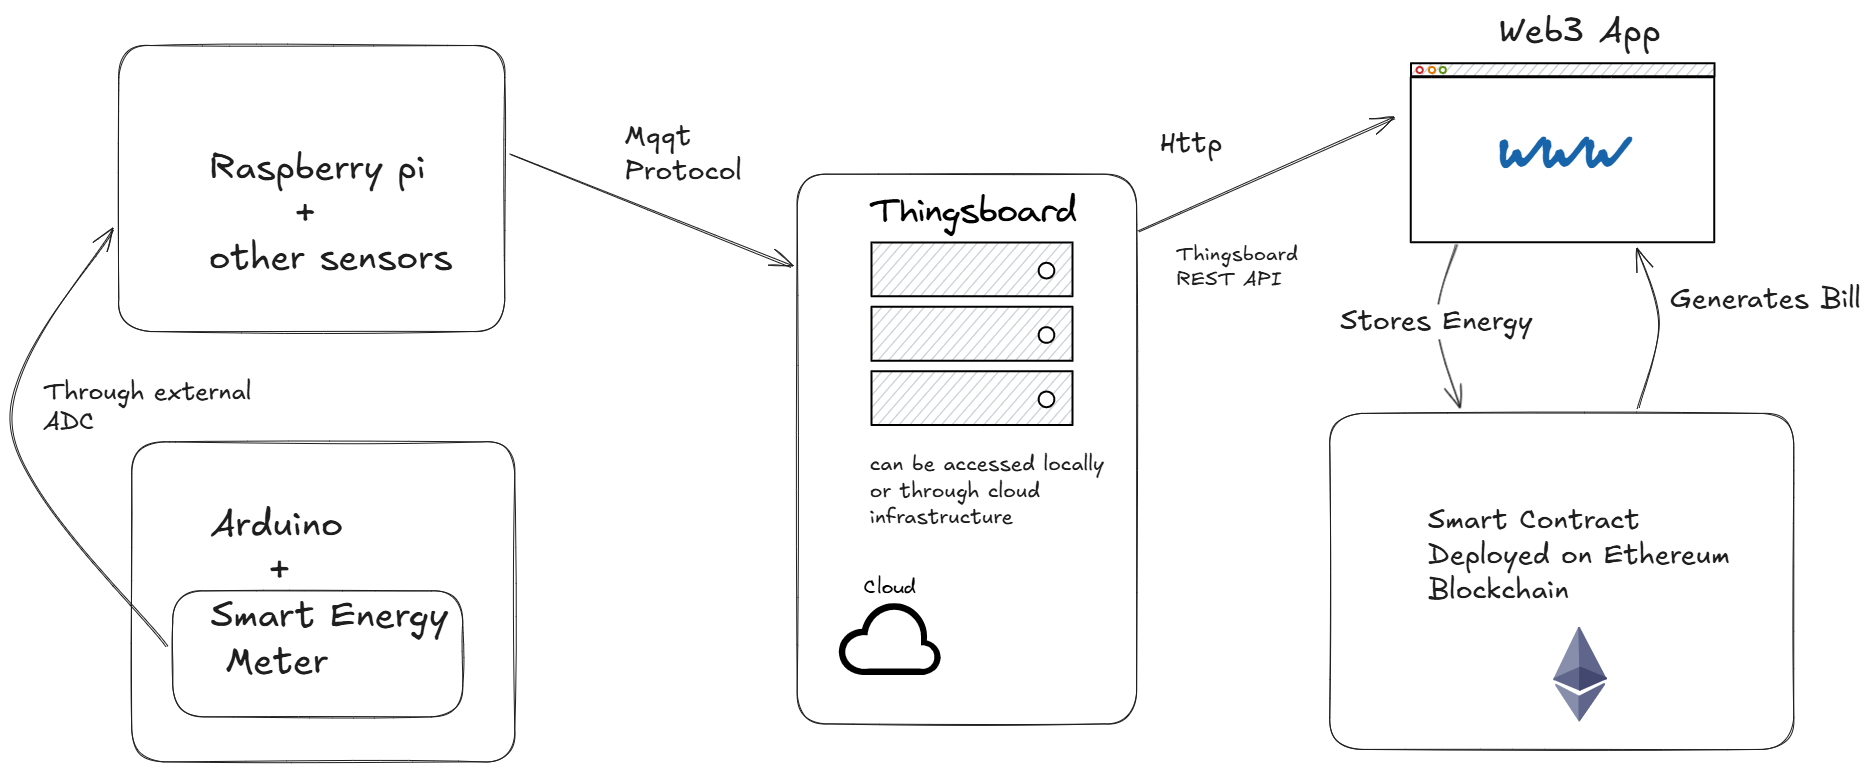
\includegraphics[width=0.9\textwidth]{basicArchitecture.png}
    \caption{System Workflow}
    \label{fig:workflow}
\end{figure}

\section{Components and Data Flow}

\subsection{Energy Measurement and Data Acquisition}

The system starts with an Arduino connected to a smart energy meter, which measures power consumption. Since Arduino lacks a built-in analog-to-digital converter (ADC) with the required resolution, an external ADC is used for accurate readings. The measured data is then transmitted to a Raspberry Pi for further processing.

\subsection{Data Transmission and Storage}

This chapter illustrates the workflow of a smart home automation system that is integrated with blockchain for energy billing.  The system's goal is to collect energy consumption data, store it in a cloud-based IoT platform, and bill and pay using a Web3 application that interacts with an Ethereum blockchain smart contract.

\subsection{Web3 Integration and Smart Contracts}

A Web3 application fetches energy consumption data from ThingsBoard via HTTP requests. The retrieved energy data is then stored in a smart contract deployed on the Ethereum blockchain. The smart contract automatically generates an energy bill based on the stored consumption values.

\subsection{Billing and Payment System}

Using HTTP queries, a Web3 application retrieves energy usage data from ThingsBoard.  A smart contract that is implemented on the Ethereum blockchain then stores the energy data that has been recovered.  Using the saved consumption values, the smart contract automatically creates an energy bill.

\section{Conclusion}

This process combines blockchain, cloud computing, and the Internet of Things to produce an automated and decentralized energy billing system.  An effective and transparent billing procedure is made possible by the modular architecture, which facilitates smooth data flow from energy monitoring to smart contract interactions.


\chapter{Proteus Schematic Design and Simulation}

\section{Introduction}
Proteus is a powerful software program that is commonly used to develop and simulate embedded systems prior to their real implementation.  It allows you to efficiently test circuits, detect design problems, and enhance performance without the need for actual hardware.  This chapter focuses on the schematic design and modeling of a smart home automation system and a smart energy meter, which integrate sensors, actuators, and communication modules to provide real-time monitoring and control.


The Raspberry Pi 3 serves as the core processing unit for the smart home automation system, which communicates with a variety of sensors such as Light Dependent Resistors (LDR), Passive Infrared (PIR) sensors, and gas detectors to automate household appliances.  The Raspberry Pi lacks built-in analog input capabilities, thus an external ADC (MCP3208) is used to interpret analog sensor data and enabling IoT-based automation\cite{valov2020home}.

The smart energy meter focuses on real-time power consumption monitoring, incorporating an Arduino Uno for data acquisition, ACS712 current sensors for current measurement, and voltage dividers for accurate voltage monitoring \cite{li2010application}. Additionally, power factor measurement is achieved using LM358 operational amplifiers and XOR gates to analyze phase differences between voltage and current waveforms \cite{Khair_2017}. These measurements are transmitted to the IoT platform, enabling remote energy management and optimization.

This chapter details the schematic design, component selection, and software implementation in Proteus.  The proposed system provides not just automation and remote monitoring, but also efficient energy utilization and billing.  Proteus simulations evaluate the system's many features prior to real-world deployment, ensuring reliability and performance.

\section{Schematic Design in Proteus}
\subsection{Smart Home Automation System}
The home automation circuit includes:

\textbf{Raspberry Pi 3:} The Raspberry Pi 3 B+ was chosen for this home automation project because of its powerful capabilities and simplicity of integration.  It is driven by a Broadcom BCM2837B0 quad-core Cortex-A53 (ARMv8) processor clocked at 1.4GHz, with 1GB LPDDR2 SDRAM and a Broadcom Videocore-IV GPU. Networking options include Gigabit Ethernet (by USB), dual-band Wi-Fi (2.4GHz and 5GHz 802.11b/g/n/ac), and Bluetooth 4.2 (BLE)\cite{valov2020home}.It includes a 40-pin GPIO header, HDMI, a 3.5mm audio connector, four USB 2.0 ports, Ethernet, CSI, and DSI.  The Micro-SD storage format and compact dimensions (82mm × 56mm × 19.5mm, 50g) make it ideal for embedded applications\cite{valov2020home}.

\begin{figure}[H]  % 'h' places the figure approximately here
    \centering
    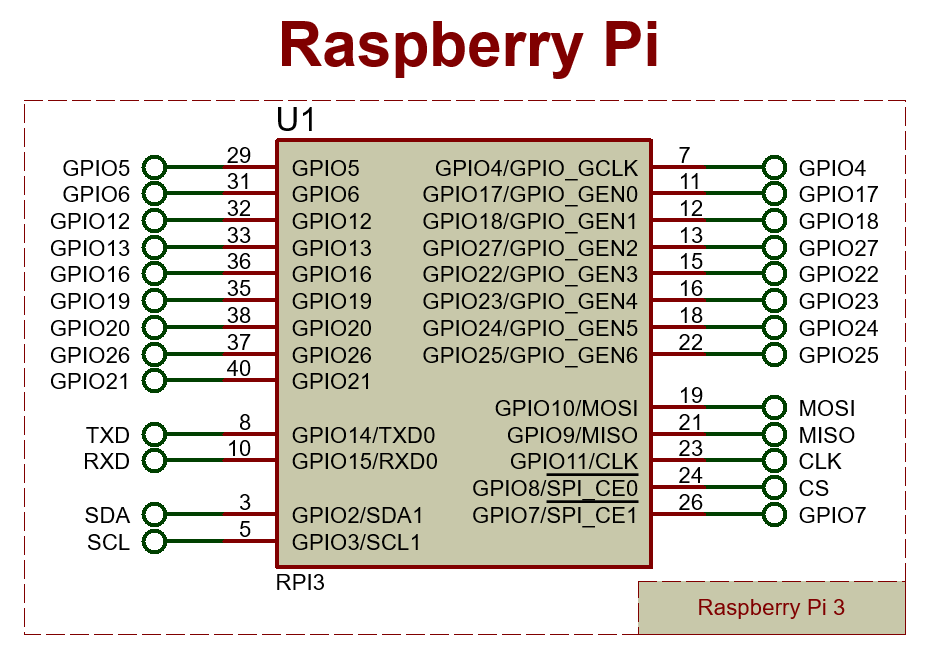
\includegraphics[width=0.6\textwidth]{image.png} % Adjust width as needed
    \caption{Raspberry Pi 3 Schematic}
    \label{fig:Raspberry} % Label for referencing the figure
\end{figure}


\textbf{ADC (MCP3208):} Analog-to-digital converters (ADCs) transform analog signals into digital data, allowing microcontrollers and computers to process real-world inputs.The MCP3208 is a 12-bit ADC with 8 input channels. It provides high accuracy (±1 LSB DNL, ±1-2 LSB INL) and low power consumption.  It runs on 2.7V-5.5V, has an SPI interface, and is commonly used for sensor applications and data gathering\cite{Dout199927V41}.

\begin{figure}[H]  % 'h' places the figure approximately here
    \centering
    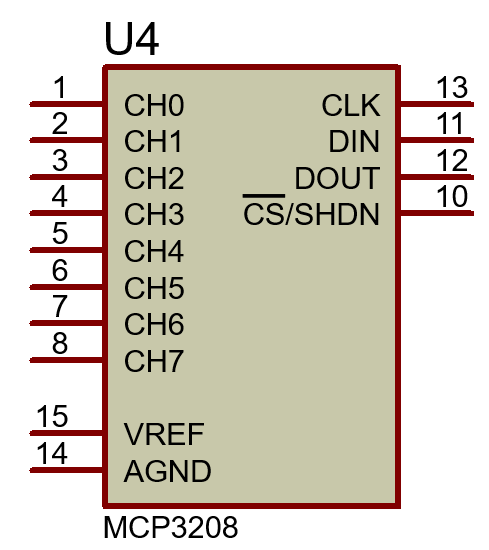
\includegraphics[scale=0.4]{MCP3208.PNG} % Adjust width as needed
    \caption{ADC (MCP3208)}
    \label{fig:adc} % Label for referencing the figure
\end{figure}

Because Raspberry Pi lacks built-in analog inputs, an external ADC such as the MCP3208 is required to read analog sensor data.  Interfacing via SPI allows for real-time monitoring in IoT applications and industrial automation\cite{Flurry2021}.

\textbf{Other Sensors:} We used a variety of sensors and actuators to allow for sophisticated control and monitoring.  The system uses an LDR (Light Dependent Resistor) to detect ambient light levels, allowing lights to be turned on or off based on the brightness of the surroundings. 
A PIR (Passive Infrared) sensor was used to detect motion and human presence.  This sensor is essential for security and automated lighting because it activates lights or alerts when motion is detected.  Furthermore, a MQ-2 gas sensor was used to monitor air quality and identify combustible gases such as LPG and CO, assuring safety by sending alarms in the event of a gas leak.  The LM35 temperature sensor was included to properly monitor room temperature and allow for automatic cooling control.

\subsection{Complete Schematic of Smart Home Automation System}
The smart home automation circuit integrates multiple sensors and actuators to automate home appliances based on environmental conditions ans involves following connections.
\begin{figure}[H]  % 'h' places the figure approximately here
    \centering
    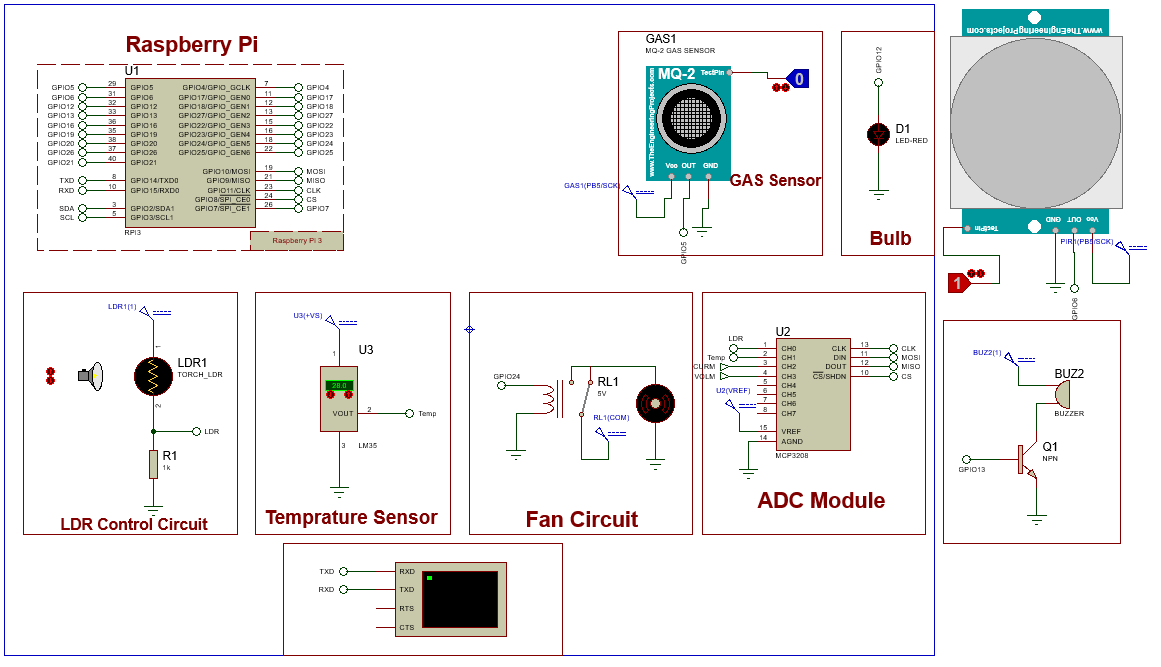
\includegraphics[scale=0.68]{smartHomeAutocomplete.PNG} % Adjust width as needed
    \caption{Complete Schematic}
    \label{fig:schematichome} % Label for referencing the figure
\end{figure}



\subsection{Smart Energy Meter and Power Factor Measurement}
The smart energy meter circuit consists of:

\textbf{Arduino Uno:}The Arduino Uno, built around the AVR microcontroller, has developed as a versatile platform for teaching and implementing digital control systems.  


\begin{figure}[H]
    \centering
    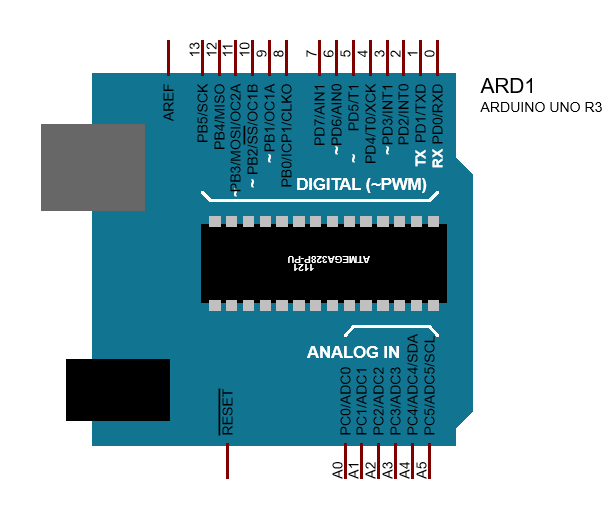
\includegraphics[width=0.6\textwidth]{Capture.PNG} % Adjust width as needed
    \caption{Arduino Uno}
    \label{fig:uno} % Label for referencing the figure

\end{figure}
It has characteristics suited for power electronics applications, providing switching frequencies of up to 100 kHz with extra libraries\cite{muller2015using}.  The Arduino Uno has been shown to be effective in controlling industrial-scale instruments, performing similarly to industrial-class controllers that use PID algorithms\cite{Taufiq_2020}.The Arduino Uno, which is based on the Atmega328 processor, supports Assembly and C programming, allowing students to learn about microcontroller architecture and interact with real-world devices like LCDs, motors, and sensors\cite{Naimi2017TheAM}. 

\textbf{Current Measurement}:In our smart home automation project, we employ the ACS712 Hall-effect-based current sensor to monitor AC/DC power levels. It has low resistance (1.2 mohm) and 2.1 kVRMS isolation for precise and safe current measuring\cite{li2010application}. The 30A variant with 66mV/A sensitivity is integrated with an arduino uno, allowing for real-time power tracking and energy consumption analysis via ThingsBoard.  Calibration improves accuracy and reduces measurement error, making it ideal for IoT-based billing and automation systems.  Its rapid reaction (5 µs) and low noise improve performance for smart energy management\cite{Khair_2017}.
\begin{figure}[H]
    \centering
    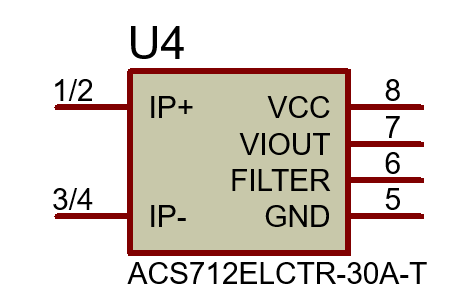
\includegraphics[width=0.35\textwidth]{ACS.PNG} % Adjust width as needed
    \caption{Current Sensor}
\end{figure}


\textbf{Voltage Measurement:}We monitor AC voltage in our smart home automation project with a step-down transformer, a voltage divider network, and a filtering capacitor. The step-down transformer (TR3) converts the high AC mains voltage to a lower, safer level suited for measurement. The voltage divider circuit (R9, R10, R11, and R12) reduces the voltage to a range compatible with the Arduino ADC, ensuring precise readings while protecting the microcontroller. A 500µF capacitor (C2) filters, reduces noise, and stabilizes the signal for accurate RMS voltage measurement. This configuration enables the Arduino to process voltage data and send it to ThingsBoard, allowing for real-time monitoring and effective energy management in our smart home system.
\begin{figure}[H]
    \centering
    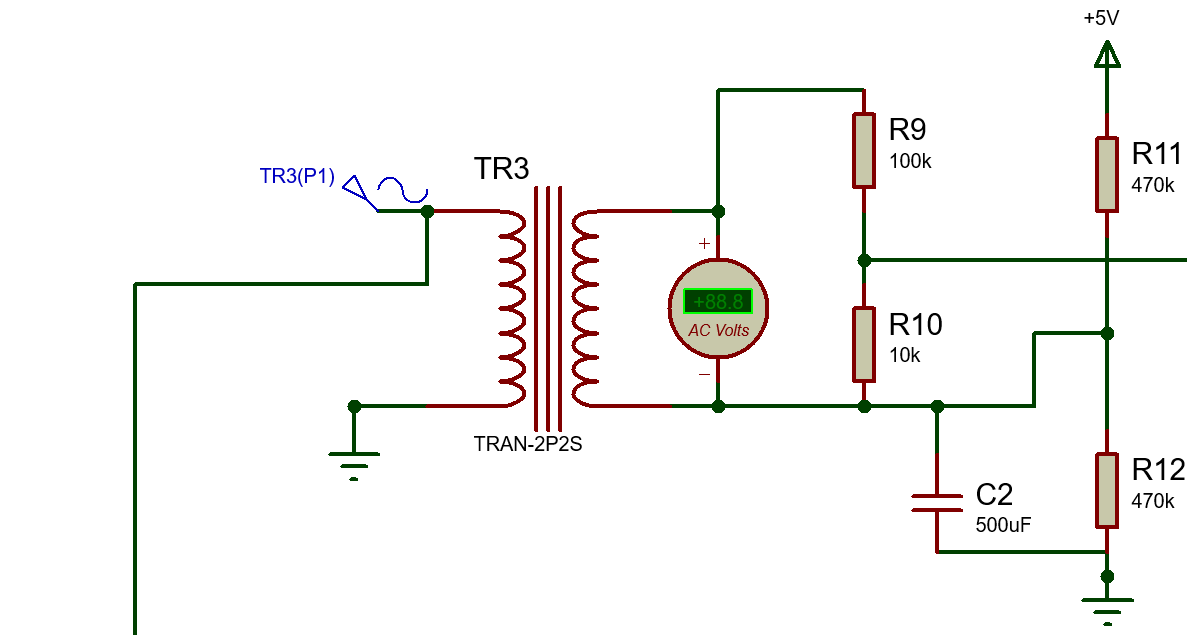
\includegraphics[width=0.6\textwidth]{voltageMeasurment.PNG} % Adjust width as needed
    \caption{Voltage Measurement Circuit}
\end{figure}

\textbf{Power Factor Measurement:} we monitor power factor with LM358 operational amplifiers and an XOR gate.  The LM358 op-amps act as zero-crossing detectors, transforming AC voltage and current waveforms to square waves.  The first op-amp (U8:A) detects zero crossings in the voltage waveform, whereas the second op-amp (U8:B) detects current waveform.  These processed signals are then routed through an XOR gate (U9), which generates a pulse-width output proportional to the phase difference between the voltage and current waves.  The Arduino measures pulse width and calculates power factor as cos($\theta$), where $\theta$ is the phase angle.
\begin{figure}[h]
    \centering
    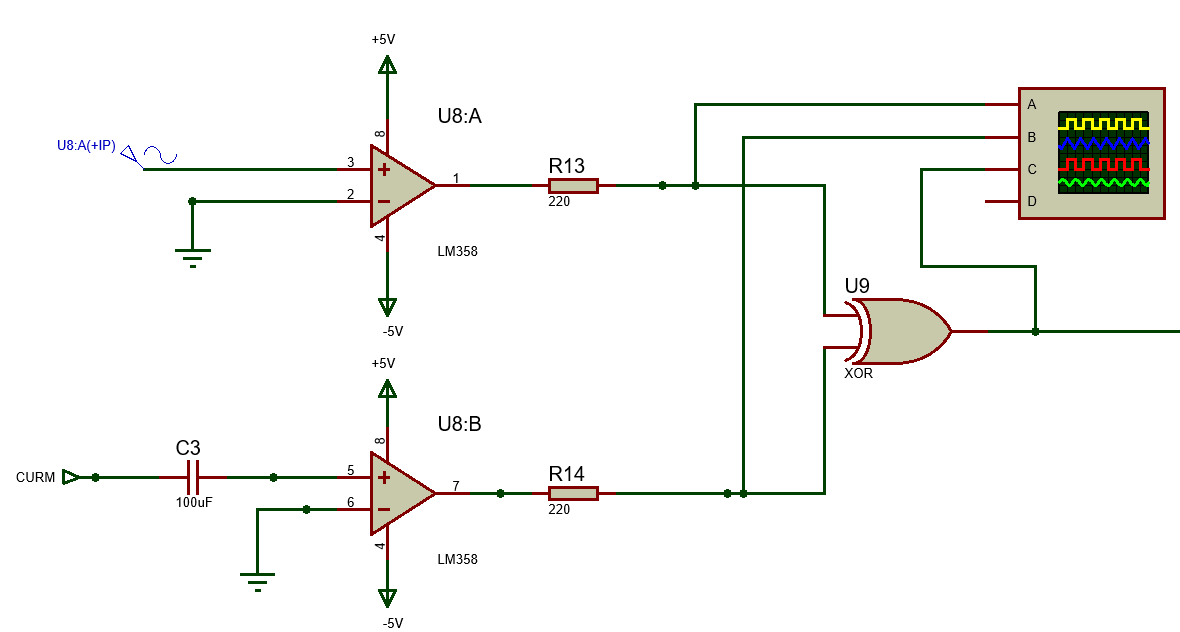
\includegraphics[width=0.6\textwidth]{PowerFactor.PNG} % Adjust width as needed
    \caption{PowerFactor Measurement Circuit}
\end{figure}

\textbf{relay-based load control} electrical appliances are managed remotely using a relay control system. The circuit consists of electromagnetic relays (RL4, RL5) that are controlled by the microcontroller's GPIO pins (for example, Raspberry Pi or Arduino). When a GPIO pin is set to HIGH, the accompanying relay coil is activated, shutting the switch and enabling current to flow to the attached load (such as lights or motors).

\subsection{Complete Schematic of Smart Energy Meter}
The smart energy meter circuit is designed to measure and monitor power consumption while ensuring efficient energy usage.
\begin{figure}[H]
    \centering
    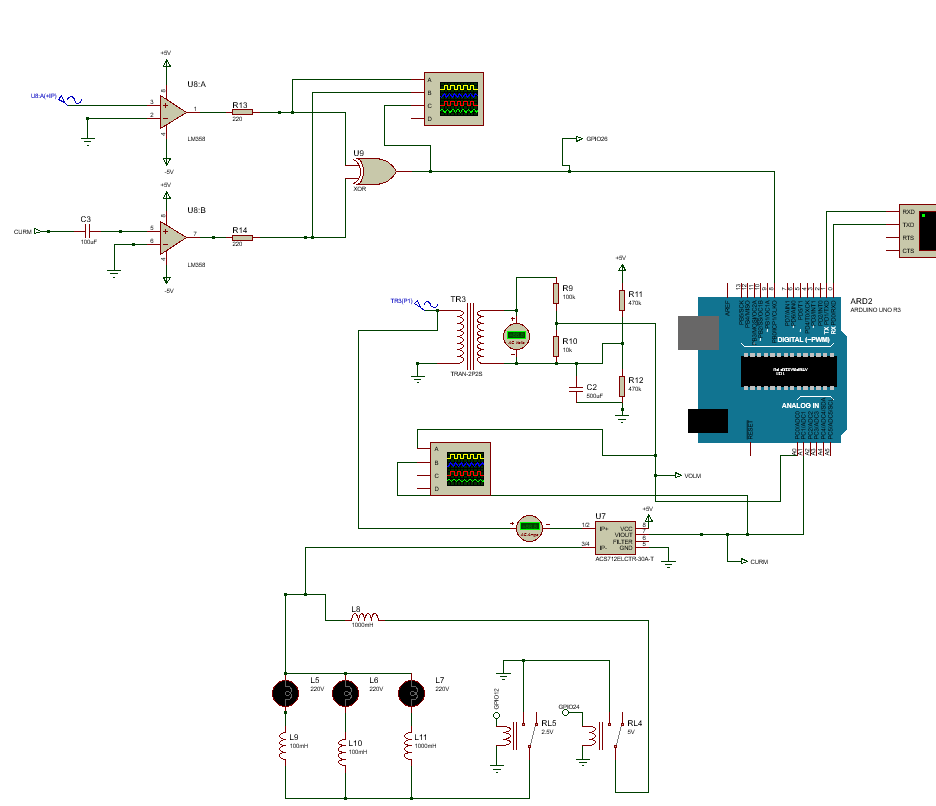
\includegraphics[width=1\textwidth]{smartEnergy.PNG} % Adjust width as needed
    \caption{Complete Schematic of Smart Energy meter}
\end{figure}

\section{Code Implementation}

\subsection{Arduino Code for Smart Energy Meter}

The Arduino is responsible for measuring voltage, current, and calculating power consumption in real-time. The analog pins read voltage and current sensor outputs, which are then converted into meaningful electrical values. The calculated power is then transmitted over serial communication.
\clearpage

\begin{lstlisting}[language=C]
// Pin configuration
const int voltagePin = A0; // Voltage sensor input
const int currentPin = A1; // Current sensor input

// Constants for sensor calibration
const float voltageMultiplier = 230.0 / 1023.0;  // Adjust based on sensor specs
const float currentMultiplier = 10.0 / 1023.0;   // Adjust for CT sensor scaling

void setup() {
    Serial.begin(9600);  // Start serial communication
}

void loop() {
    // Read raw analog values from sensors
    int rawVoltage = analogRead(voltagePin);
    int rawCurrent = analogRead(currentPin);
    
    // Convert raw values to real-world measurements
    float voltage = rawVoltage * voltageMultiplier;
    float current = rawCurrent * currentMultiplier;
    float power = voltage * current; // Active power calculation

    // Print the measurements to serial monitor
    Serial.print("Voltage: "); Serial.print(voltage); Serial.print(" V, ");
    Serial.print("Current: "); Serial.print(current); Serial.print(" A, ");
    Serial.print("Power: "); Serial.print(power); Serial.println(" W");

    delay(1000);  // Wait 1 second before next reading
}
\end{lstlisting}


\subsection{Raspberry Pi Code for Home Automation}

The Raspberry Pi is responsible for reading sensor data, controlling home appliances based on environmental conditions, and sending data to an IoT platform (ThingsBoard) using MQTT.
\clearpage

\begin{lstlisting}[language=Python]
import RPi.GPIO as GPIO
import time
import json
import spidev
import math
from paho.mqtt.client import Client

# GPIO setup
GPIO.setmode(GPIO.BCM)
GPIO.setup(17, GPIO.IN)  # LDR sensor for light detection
GPIO.setup(27, GPIO.OUT) # Relay control for light switching

# SPI setup for ADC communication (e.g., MCP3008)
spi = spidev.SpiDev()
spi.open(0, 0)
spi.max_speed_hz = 1350000

# MQTT setup
THINGSBOARD_HOST = "localhost"
ACCESS_TOKEN = "your_access_token"
client = Client()
client.username_pw_set(ACCESS_TOKEN)
client.connect(THINGSBOARD_HOST, 1883, 60)

# Read ADC channel for sensor values
def read_channel(channel):
    adc = spi.xfer2([1, (8 + channel) << 4, 0])
    return ((adc[1] & 3) << 8) + adc[2]

# Calculate RMS voltage from multiple samples
def calculate_rms_voltage():
    sum_squares = sum((read_channel(3) * 3.3 / 1023.0) ** 2 for _ in range(200))
    return math.sqrt(sum_squares / 200) * 11  # Voltage divider correction

# Publish sensor data to MQTT
def publish_sensor_data():
    while True:
        light_level = read_channel(0)  # Read LDR sensor value
        GPIO.output(27, light_level < 100)  # Turn on relay if dark
        
        payload = json.dumps({
            "light": light_level,
            "voltage": calculate_rms_voltage()
        })
        client.publish("v1/devices/me/telemetry", payload)
        time.sleep(0.5)  # Wait before next update

publish_sensor_data()
\end{lstlisting}

\section{Simulation and Testing}

\subsection{Home Automation Testing}
Several tests were run in the Proteus simulation environment to validate the smart home automation system.  The LDR-based light control circuit was tested under various lighting situations.  The simulation confirmed that when the light intensity fell below a particular threshold, the relay was activated, which turned on the linked bulb.  When the light intensity increased, the relay deactivated and the bulb turned off.  This behavior provided automatic lighting management based on ambient light levels.

 The PIR sensor was tested by mimicking motion within its detecting range.  When motion was detected, the buzzer sounded an alert.  When there was no motion, the buzzer remained off.  This proved that the motion detection system was working properly, making it appropriate for security applications.


The MQTT communication between the Raspberry Pi and ThingsBoard Cloud was also tested. Sensor data, including light intensity and relay state, was successfully transmitted and displayed on the ThingsBoard dashboard in real time. This validated the proper integration of IoT communication in the system.

\subsection{Smart Meter Testing}
The smart energy meter system was evaluated for accuracy and dependability in measuring electrical characteristics.  The Arduino successfully obtained voltage and current readings from the sensors.  These readings were compared to expected values, and the findings revealed an acceptable margin of error, indicating measurement accuracy.

The power consumption was calculated using the formula \( P = V \times I \), and the computed values were displayed on the serial monitor. The readings matched theoretical expectations, demonstrating the correct implementation of power measurement.

Furthermore, the power factor correction circuit was simulated by adding different loads.  As reactive power varied, the circuit modified to enhance the power factor.  This enabled the system to dynamically optimize power consumption, decreasing energy waste.


\section{Conclusion}

The Proteus simulation offered a dependable testing environment for both the smart home automation and smart energy metering systems.  The home automation system operated as planned, automatically regulating lighting based on ambient conditions and detecting motion to trigger security warnings.  The smart meter measured electrical characteristics precisely and estimated power usage with excellent reliability. 

 Both systems' successful simulation testing shows that they are ready for real-world implementation.  With the right hardware, these systems can improve energy efficiency and automation in smart home situations.


\chapter{ThingsBoard Integration}
\section{Introduction to ThingsBoard}
Rapid breakthroughs in semiconductor technology and wireless communication have resulted in the development of low-cost sensor-based devices, which serve as the foundation for the Internet of Things (IoT) ecosystem\cite{estrin1999next}.  These sensors produce massive volumes of data, demanding effective collection, processing, and management frameworks.  IoT platforms play an important role in managing this data by offering connectivity, security, data visualization, and analytics capabilities\cite{hammi2018iot}\cite{gazis2015survey}.  Among these platforms, ThingsBoard has emerged as an effective open-source solution for IoT data collecting and management.

ThingsBoard is a Java 8-based IoT platform that acts as a gateway for devices that communicate using MQTT\cite{kegenbekov2022using}, CoAP\cite{shelby2014rfc}, and HTTP\cite{yassein2016application}.  These protocols allow for lightweight communication between resource-constrained IoT devices and cloud services.  MQTT is a publish/subscribe protocol for small, low-power devices that enables efficient message exchange via a broker with varying Quality of Service (QoS) levels\cite{kegenbekov2022using}.  In contrast, CoAP is an UDP-based protocol designed for limited contexts, with lower overhead but lesser dependability than MQTT\cite{shelby2014rfc}.
One of ThingsBoard's key features is the ability to build rules and plugins for message processing.  Rules contain data filters, metadata enrichment processors, and action triggers that change messages into new formats before sending them to plugins.  This rule-based system supports basic data processing, including threshold-based notifications.  However, the technology does not automatically support complex data aggregation over time or across several devices\cite{hammi2018iot}.

 ThingsBoard allows you to configure alerts for both devices and assets, which improves real-time monitoring and event-based automation.  When aberrant situations are recognized, these alerts alert users or initiate automated replies.  Furthermore, the platform supports both lightweight communication protocols, such as MQTT and CoAP, and classic RESTful services\cite{shelby2014rfc}. 

 \begin{figure}[H]
    \centering
    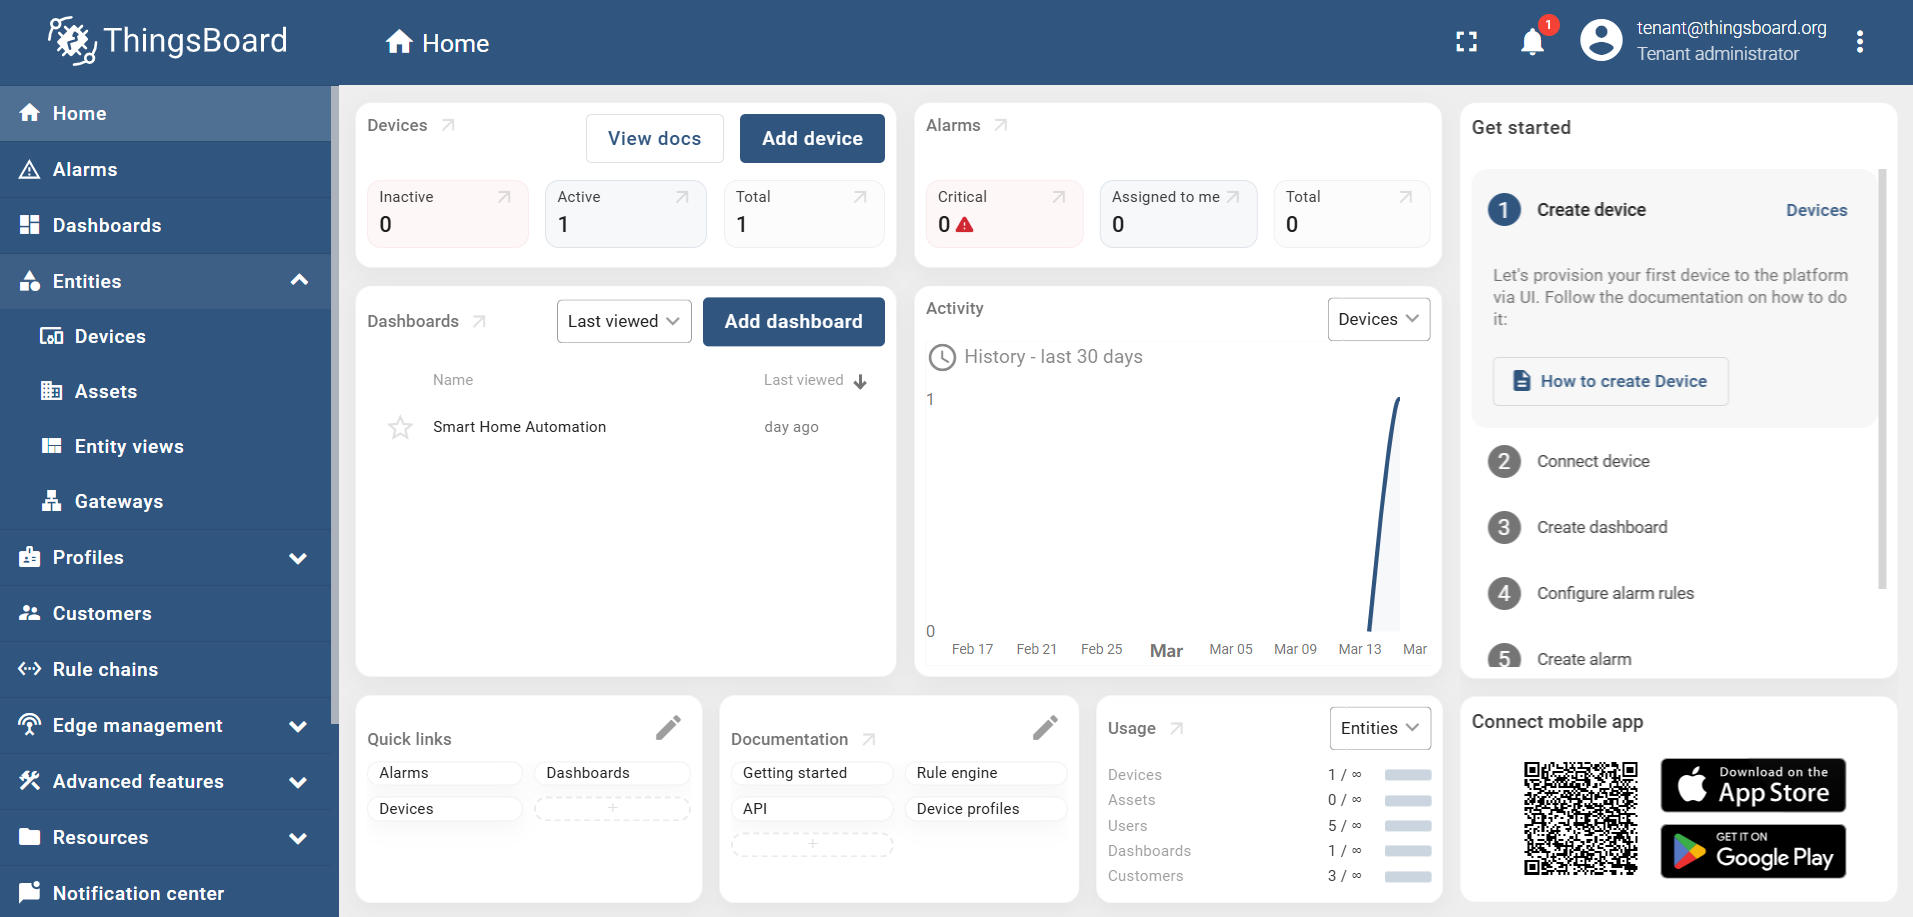
\includegraphics[width=1\textwidth]{home.PNG}
    \caption{ThingsBoard's Home}
 \end{figure}

 \section{Prerequisites for ThingsBoard MQTT Integration}

 Before integrating ThingsBoard with MQTT, ensure that the required software components are installed and configured correctly. The ThingsBoard platform must be running on either a local system or a cloud server. Although ThingsBoard has a built-in MQTT broker, an external broker such as Mosquitto can also be used if needed.Each device must first be created in ThingsBoard before it can communicate via MQTT. To create a new device, navigate to the ThingsBoard dashboard, go to the \textbf{Devices} section, and click on \textbf{Add New Device}. Assign a meaningful name and select the appropriate device type. Once the device is created, an \textbf{Access Token} is generated, which will be required for authentication in MQTT communication. A visual representation of the device creation process is shown in Figure~\ref{fig:device_creation}. Additionally, MQTT communication requires appropriate network settings. Ensure that port \textbf{1883} is open for unencrypted communication. Each device must authenticate with ThingsBoard using an \textbf{Access Token}, which is assigned when the device is created in ThingsBoard.
 
 \begin{figure}[H]
    \centering
    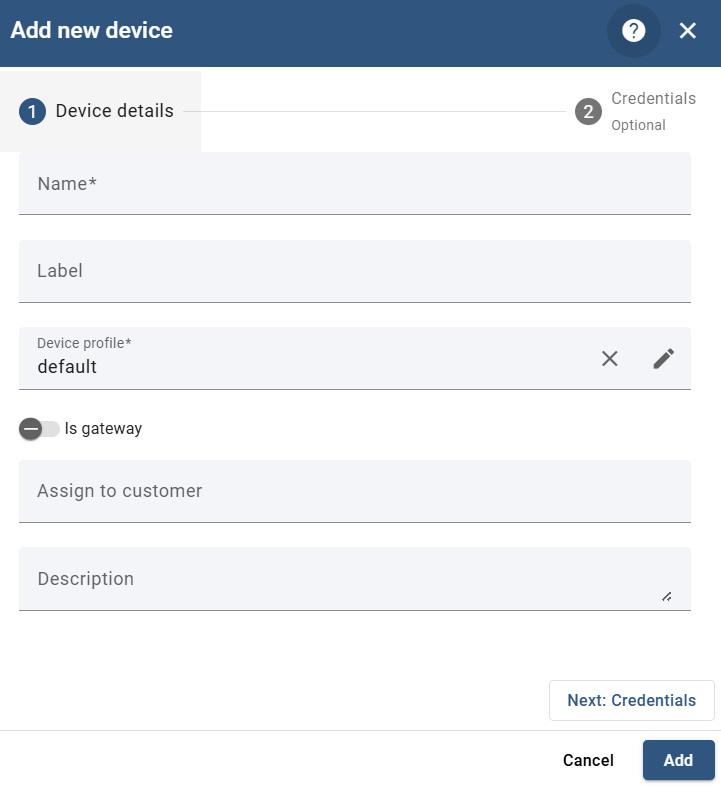
\includegraphics[width=0.35\textwidth]{device creation.PNG}
    \caption{Device creation process in ThingsBoard}
    \label{fig:device_creation}
 \end{figure}

 
 \section{Connecting ThingsBoard with MQTT}
 
 To send telemetry data to ThingsBoard using MQTT, follow these steps:
 
 \subsection{Step 1: Define Connection Parameters}
 The first step is to configure the MQTT connection by specifying the ThingsBoard host, access token, and MQTT port. Replace the \texttt{ACCESS\_TOKEN} with the token obtained from the ThingsBoard device.
 
 \begin{lstlisting}
 THINGSBOARD_HOST = "localhost"
 ACCESS_TOKEN = "dU6S0YIAPX5WwfmB3wUi"  # Replace with your actual token
 MQTT_PORT = 1883
 \end{lstlisting}
 
 \subsection{Step 2: Install and Import MQTT Library}
 After setting up the connection parameters, ensure that the \texttt{paho-mqtt} library is installed. This library is required to establish an MQTT connection. Once installed, import the necessary modules in the Python script.
 
 \begin{lstlisting}
 import paho.mqtt.client as mqtt
 import json
 \end{lstlisting}
 
 \subsection{Step 3: Create MQTT Client and Connect}
 The next step is to create an MQTT client instance and authenticate using the access token. The client must then connect to the ThingsBoard host on the specified port.
 
 \begin{lstlisting}
 client = mqtt.Client()
 client.username_pw_set(ACCESS_TOKEN)  # Use Access Token for authentication
 client.connect(THINGSBOARD_HOST, MQTT_PORT, 60)
 \end{lstlisting}
 
 \subsection{Step 4: Publish Sensor Data}
 Once connected, sensor data must be prepared in JSON format and published to the ThingsBoard MQTT topic. The following code snippet demonstrates how to send temperature and humidity data.
 
 \begin{lstlisting}
 telemetry_data = {"current": 14.919, "fan_status": 0,"gas_detected":0,"light":61,"motion":1,"power":3493.48,"power_factor":0.98,"temperature":27.85}
 client.publish("v1/devices/me/telemetry", json.dumps(telemetry_data))
 print("Data sent successfully!")
 client.disconnect()
 \end{lstlisting}

 \begin{figure}[H]
    \centering
    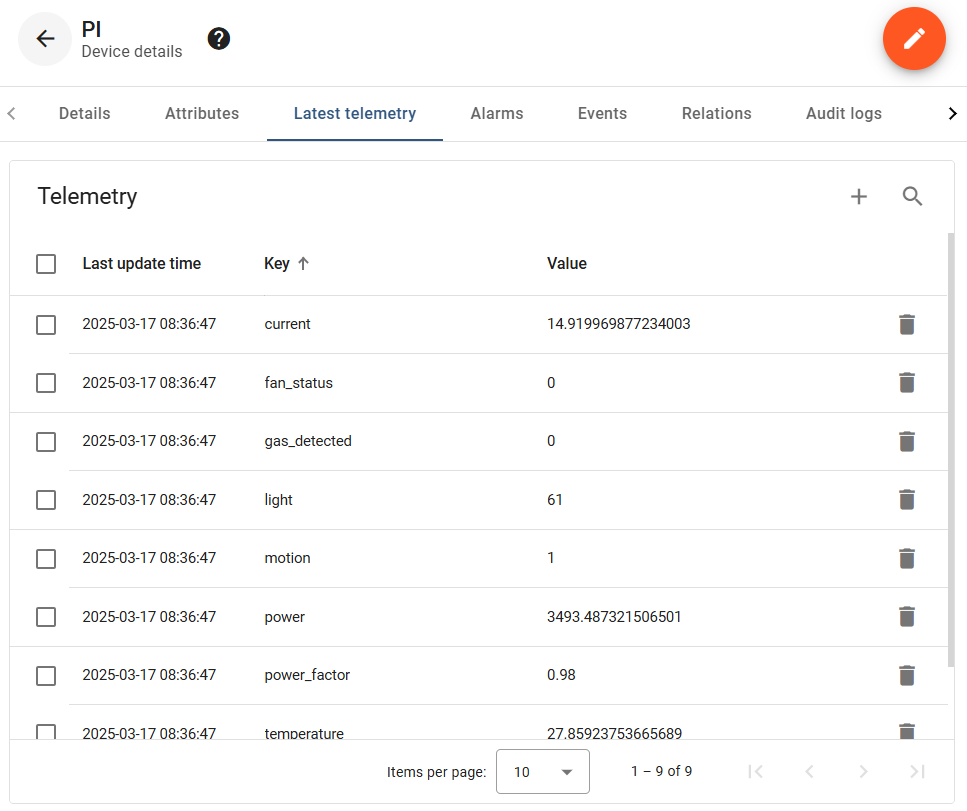
\includegraphics[width=0.8\textwidth]{device Details.PNG}
    \caption{Latest Telemetry after Publishing Data}
 \end{figure}
 
 \subsection{Step 5: Verify Data in ThingsBoard}
 After publishing the data, it is essential to verify whether ThingsBoard has received it. This can be done by navigating to the ThingsBoard UI and checking the \textbf{Latest Telemetry} section of the configured device.

 \subsection{Step 6:Creation of Dashboard in ThingsBoard}
 After creating a device in ThingsBoard, the next step is to create a dashboard for monitoring and visualization. To create a new dashboard, navigate to the \textbf{Dashboards} section and click on \textbf{Create New Dashboard}. Provide a meaningful name and description for easy identification.

 Once the dashboard is created, widgets can be added to visualize device telemetry data. Click on \textbf{Edit Dashboard}, then use the \textbf{Add New Widget} option to select an appropriate widget type, such as charts, gauges, or tables. Link the widget to the corresponding device and telemetry keys. The dashboard creation process is illustrated in Figure~\ref{fig:dashboard_creation2}.
 \begin{figure}[H]
    \centering
    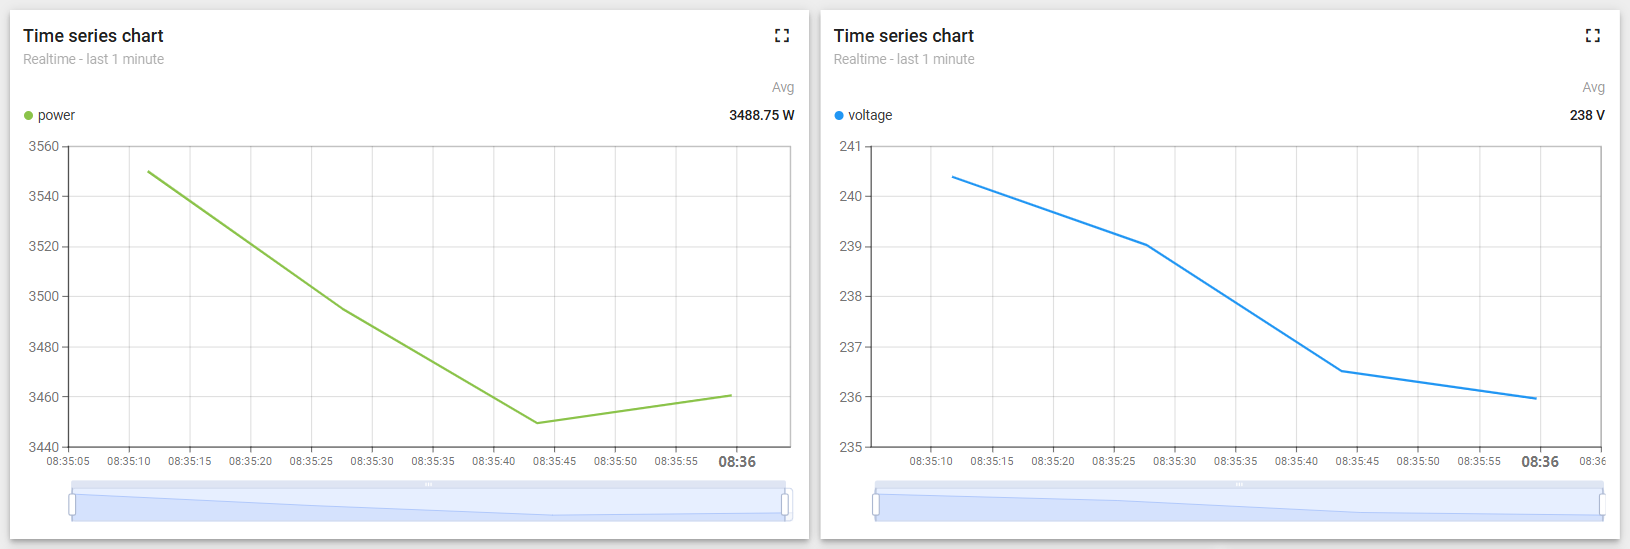
\includegraphics[width=1\textwidth]{dashboard2.PNG}
 \end{figure}
 \begin{figure}[H]
    \centering
    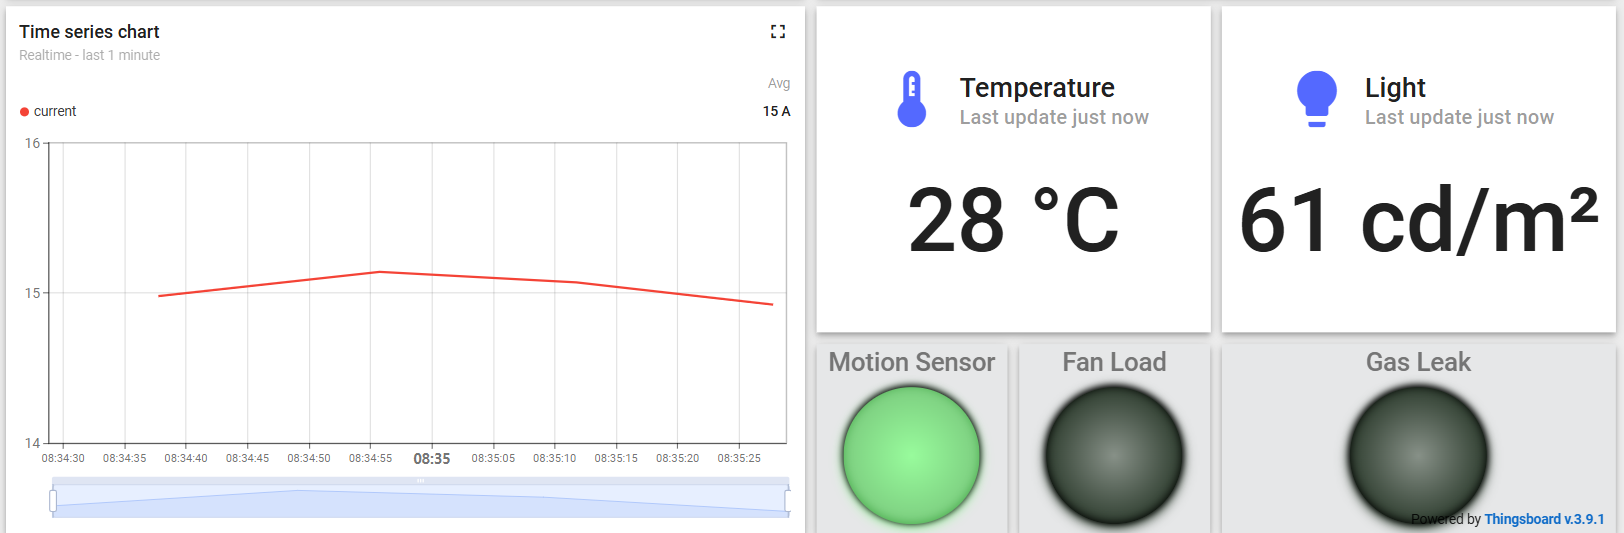
\includegraphics[width=1\textwidth]{dashboard1.PNG}
    \caption{Dashboard Creation with ThingsBoard Widgets}
    \label{fig:dashboard_creation2}
 \end{figure}
 \section{Prerequisites for ThingsBoard API Integration}
 
 Before integrating ThingsBoard with the API, ensure that the required software and authentication mechanisms are set up properly. The ThingsBoard platform must be installed on a local system or a cloud server to facilitate communication. A REST client such as Postman or the \texttt{fetch} API in JavaScript is necessary for interacting with ThingsBoard’s API. Additionally, proper network access should be configured to allow API requests.
 
 To ensure security, ThingsBoard requires authentication via a JSON Web Token (JWT). The authentication process involves sending a username and password to ThingsBoard’s login API. Upon successful authentication, a token is generated, which must be included in all subsequent API requests. Without this token, ThingsBoard will deny access to its resources.
 
 \section{Connecting to ThingsBoard API}
 
 To fetch telemetry data from ThingsBoard, follow these steps:
 
 \subsection{Step 1: Generate Access Token}
 The first step is to authenticate with ThingsBoard and obtain an access token. This is done by sending a POST request to the authentication API with valid credentials. The request should be formatted in JSON, containing a username and password.
 
 \begin{lstlisting}
 POST http://localhost:9090/api/auth/login
 Content-Type: application/json
 
 {
     "username": "tenant@thingsboard.org",
     "password": "tenant"
 }
 \end{lstlisting}
 
 \subsection{Step 2: Extract JWT Token}
 Once the authentication request is processed, the API will return a response containing a JWT token. This token is essential for making authorized requests to ThingsBoard. The response will be in JSON format, and the token can be extracted from the \texttt{token} field.
 
 \begin{lstlisting}
 {
     "token": "eyJhbGciOiJIUzI1NiIsInR5cCI...",
     "refreshToken": "eyJhbGciOiJIUzI1NiIsIn..."
 }
 \end{lstlisting}
 
 \subsection{Step 3: Fetch Telemetry Data}
 After obtaining the authentication token, the next step is to retrieve telemetry data from a specific device. The device ID must be specified in the request URL, and the JWT token must be included in the request headers under the \texttt{X-Authorization} field. The following JavaScript code demonstrates how to fetch power telemetry data from a ThingsBoard device.
 
 \begin{lstlisting}
 const response = await fetch( 
     `http://localhost:9090/api/plugins/telemetry/DEVICE/0eb8ae80-ffe6-11ef-b36a-71656502eb9c/values/timeseries?keys=power`,
     {
         headers: { "X-Authorization": `Bearer ${thingsboardToken}` },
     }
 );
 const data = await response.json();
 console.log(data);
 \end{lstlisting}
 
 \subsection{Step 4: Process Response Data}
 Once the telemetry data is retrieved, it will be returned in JSON format. The response will contain key-value pairs representing the requested telemetry values. The received data can then be processed, displayed, or stored as needed, depending on the application requirements.
 \section{Conclusion}
 Integrating ThingsBoard with MQTT allows for efficient and secure real-time data transmission for IoT devices. By following the methods mentioned, devices can authenticate, publish telemetry data, and take advantage of ThingsBoard's monitoring and automation capabilities. This lightweight and scalable strategy improves IoT installations by providing consistent connectivity while also allowing for future enhancements such as encryption and improved data handling.

\chapter{Blockchain and Smart Contracts}
\section{Introduction to Blockchain}
Blockchain is a fast developing technology for safe, transparent, and decentralized data management. It is based on three core components: private key cryptography, peer-to-peer networking, and smart contracts\cite{swan2016blockchain}. Transactions are encrypted with cryptographic keys, validated by distributed nodes, and kept immutably, making blockchain immune to fraud and illegal changes\cite{tern2021survey}.
Initially, blockchain was largely utilized for peer-to-peer financial transactions, as demonstrated by Bitcoin.  However, in 2013, Ethereum launched smart contracts, which allow for the automatic implementation of agreements without the use of middlemen\cite{yuan2018shadoweth}.  These self-executing contracts specify the terms and circumstances of a transaction while ensuring efficiency, security, and dependability\cite{falazi2020smart}.

 Smart contracts have transformed businesses by allowing for smooth transactions in fields such as finance, supply chain management, and digital asset exchanges.  By eliminating intermediaries, they save money, boost transparency, and build confidence among participants\cite{johari2021smart}.  Blockchain and smart contracts are becoming increasingly popular, opening up new opportunities for safe and efficient digital transactions.



 \section{Advantages of Blockchain and Smart Contracts}
 Blockchain technology offers numerous advantages, including decentralization, security, transparency, and immutability. Since blockchain operates on a distributed ledger, there is no single point of failure, reducing the risk of downtime and attacks. Transactions recorded on the blockchain are secure due to cryptographic hashing, ensuring data integrity. Transparency is another key advantage, as all transactions are publicly verifiable and tamper-proof. Additionally, blockchain eliminates intermediaries, making financial transactions more efficient and cost-effective.
 
 Smart contracts further enhance the blockchain ecosystem by automating and enforcing agreements without requiring intermediaries. They execute predefined conditions and ensure that transactions occur only when the conditions are met. This eliminates the need for third parties such as banks, legal entities, or brokers, thus reducing costs and increasing efficiency. Smart contracts also provide trust and security as they are immutable once deployed on the blockchain.
 
 \section{Solidity Basics}
 Solidity is a high-level programming language used for writing smart contracts on Ethereum. It is statically typed and influenced by JavaScript, Python, and C++. Solidity contracts consist of state variables, functions, events, and modifiers. 
 
 \section{Smart Contract Deployed in the Project}
 Below is an example of a Solidity smart contract implementing an energy billing system:
 
 \begin{lstlisting}
 // SPDX-License-Identifier: MIT
 pragma solidity ^0.8.0;
 
 contract EnergyBilling {
     address public owner;
     mapping(address => uint256) public userEnergy; // Stores energy consumption per user
     mapping(address => uint256) public userBills; // Stores the bill amount per user
 
     uint256 public constant RATE_PER_KWH = 2; // Cost per kWh (Example: 2 Wei per kWh)
 
     event EnergyStored(address indexed user, uint256 energy);
     event BillPaid(address indexed user, uint256 amount);
 
     modifier onlyOwner() {
         require(msg.sender == owner, "Only owner can call this function");
         _;
     }
 
     constructor() {
         owner = msg.sender; // Set contract deployer as owner
     }
 
     function storeEnergy(uint256 _totalEnergy) public {
         require(_totalEnergy > 0, "Energy must be greater than zero");
 
         userEnergy[msg.sender] += _totalEnergy;
         userBills[msg.sender] = userEnergy[msg.sender] * RATE_PER_KWH;
 
         emit EnergyStored(msg.sender, _totalEnergy);
     }
 
     function getBill() public view returns (uint256) {
         return userBills[msg.sender];
     }
 
     function payBill() public payable {
         uint256 billAmount = userBills[msg.sender];
         require(msg.value == billAmount, "Incorrect payment amount");
 
         userBills[msg.sender] = 0; // Reset bill after payment
 
         emit BillPaid(msg.sender, msg.value);
     }
 }
 \end{lstlisting}
 
 This contract allows users to store their energy consumption, calculate their bill, and make payments. It ensures security and automation of energy billing transactions.
 
 \section{Ethereum and Gas Estimation}
 Ethereum is a decentralized platform for smart contract execution. It uses Ether (ETH), the network's currency. To execute a smart contract, users must pay gas fees, which compensate miners for their computational efforts. Gas costs vary depending on network congestion and contract complexity.
 
 Each operation in Solidity has a distinct gas cost. For example, storing data on-chain is more expensive than performing computations. Gas estimation helps developers optimize contracts by identifying operations that consume excessive gas. Tools such as Remix IDE and Ethereum testnets provide gas estimation functionality to improve contract efficiency. A visual representation of gas estimation in Remix IDE is shown in Figure~\ref{fig:gas_estimation}.
 
 \begin{figure}[H]
 \centering
 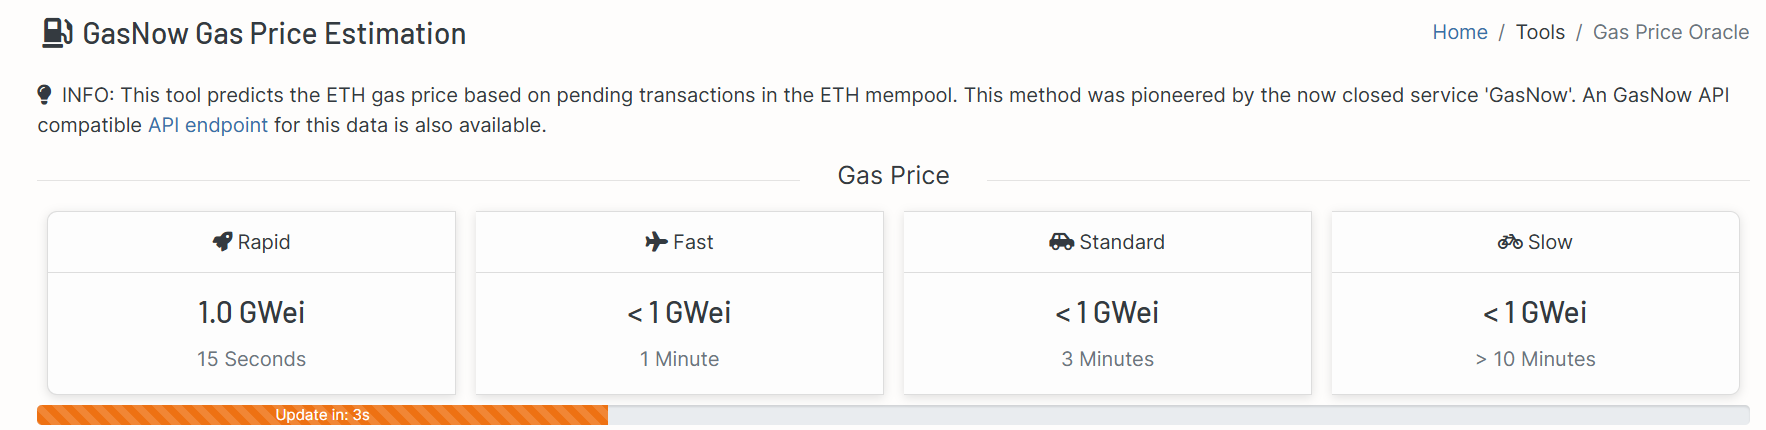
\includegraphics[width=1\textwidth]{gas price.PNG}
 \caption{Gas Tracker for Ethereum Sepolia}
 \label{fig:gas_estimation}
 \end{figure}
 
 \section{Remix IDE and Smart Contract Deployment}
 Remix IDE is an online development environment for creating, building, deploying, and debugging smart contracts. It features a user-friendly interface and built-in Solidity compiler support, allowing developers to write and test contracts efficiently.
 
 Remix also supports gas estimation, transaction debugging, and integration with Ethereum testnets. Developers can use Remix to deploy smart contracts, simulate transactions, and optimize gas usage before deploying them to the Ethereum mainnet. The deployment process in Remix IDE is illustrated in Figure~\ref{fig:remix_deployment}.
 
 \begin{figure}[H]
 \centering
 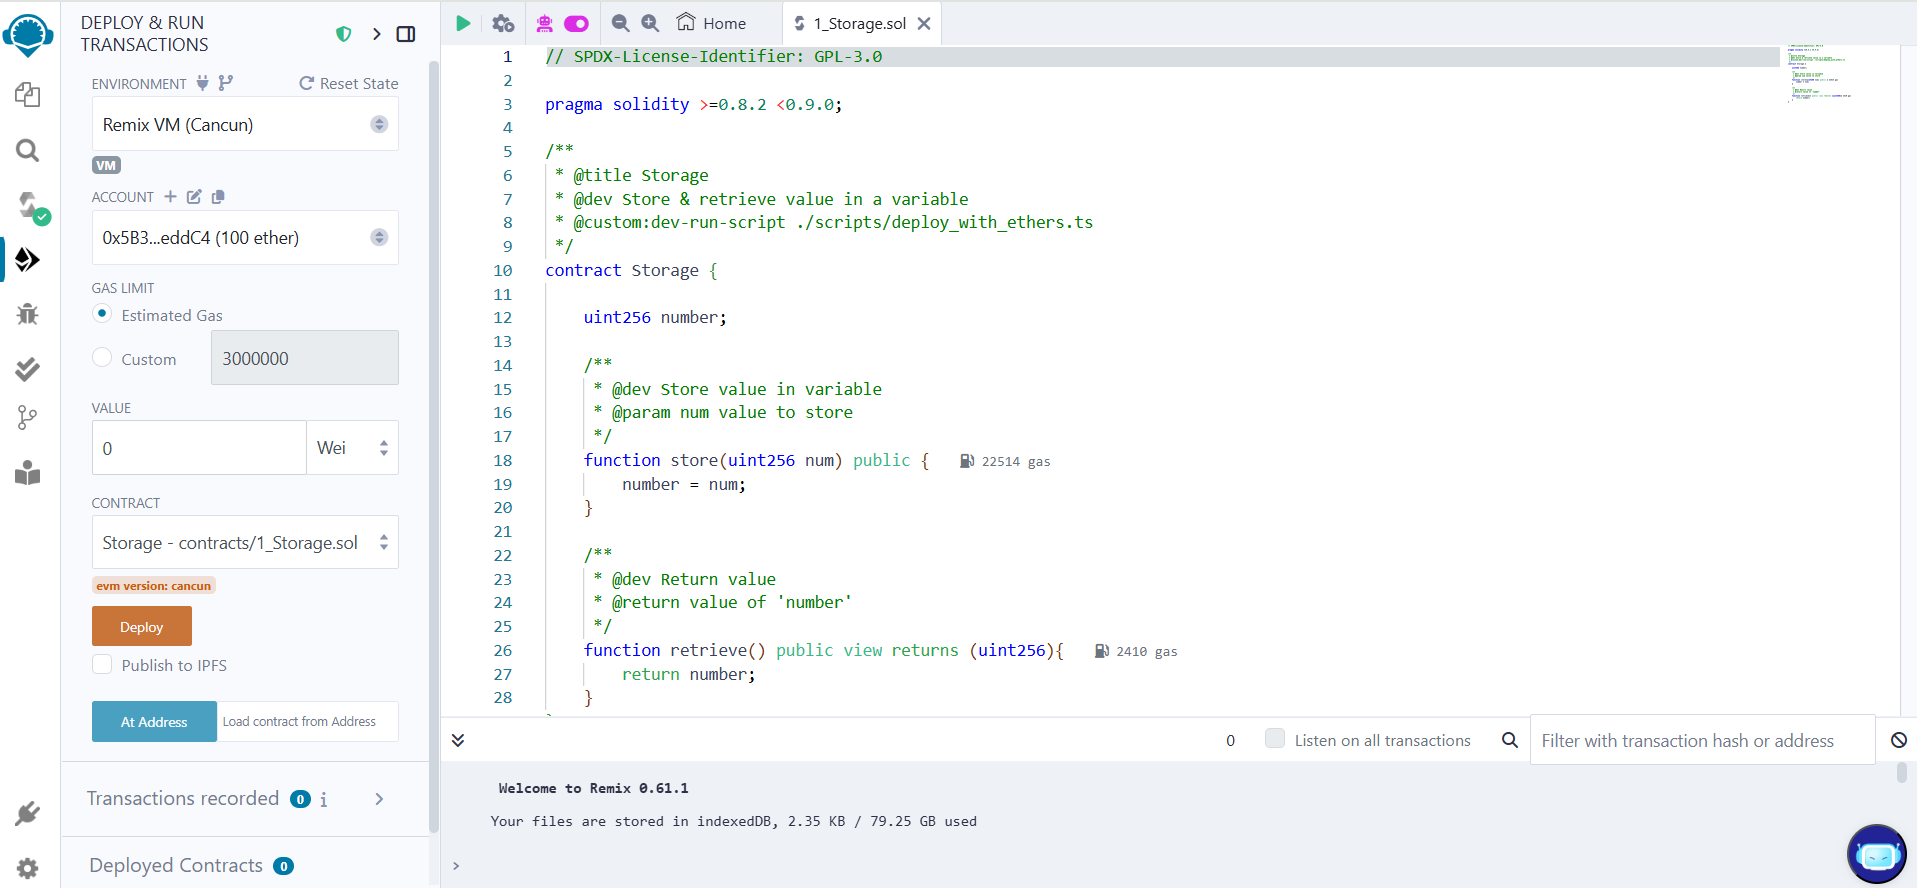
\includegraphics[width=0.8\textwidth]{remix ide.PNG}
 \caption{Smart contract deployment in Remix IDE}
 \label{fig:remix_deployment}
 \end{figure}


 \section{Conclusion}
 Blockchain and smart contracts offer a secure and decentralized method to automation across a variety of industries, including energy bills.  Solidity allows for efficient contract construction, while Ethereum provides decentralized execution using gas estimation algorithms.  Tools like Remix IDE make smart contract deployment easier, and combining IoT and blockchain improves automation and transparency in energy management.  The combination of these technologies provides the door for a more efficient and secure system for handling digital transactions and automation.

  

 \chapter{Ganache Toolchain}

\section{Introduction to Ganache}
Ganache is a personal Ethereum blockchain designed for testing and development.  It offers developers a local blockchain environment in which to build, test, and debug smart contracts before distributing them to a public or test network\cite{brightwell2015overview}.  Ganache is offered in two flavors: Ganache UI, which has a graphical interface, and Ganache CLI, a command-line tool for automation and scripting\cite{gibson2016review}.  It supports quick transactions, chain forking, and complete logging, making it a crucial tool for Ethereum development and testing\cite{wang2017review}.

One of the primary benefits of Ganache is its ability to mine transactions instantly.  Unlike public testnets, which require confirmation time, Ganache handles transactions immediately, allowing for faster iterations during development.  It also offers pre-funded accounts, making it simple to test transactions without spending real or test ETH.  Furthermore, Ganache enables developers to change network characteristics like as gas price, block time, and transaction speed, providing greater flexibility for testing various scenarios.

\section{Ethereum Testnets and Their Challenges}
Ethereum testnets, such as Sepolia, Goerli, and Holesky, allow developers to test their smart contracts before releasing them to the Ethereum mainnet.  These testnets imitate real-world Ethereum settings, such as transaction processing, block validation, and gas fees, without incurring any monetary charges.

 Sepolia is now the most popular testnet for testing smart contracts.  However, one of the most difficult aspects of using Ethereum testnets is obtaining test ETH, which is needed to deploy contracts and execute transactions.  Unlike a local blockchain, such as Ganache, testnets require developers to request ETH from faucets, which are frequently unstable or have limited availability.  Furthermore, mining test ETH on proof-of-stake testnets such as Sepolia is impossible, forcing developers to rely on third-party sources.


Another limitation of testnets is the network congestion and transaction confirmation time. Since multiple developers use these networks simultaneously, transactions may take longer to be confirmed, especially during high activity periods. This delays testing and debugging, making it harder to iterate quickly on smart contract development.

\section{Why Ganache is Beneficial for Development}
Ganache offers a speedier, more regulated, and cost-effective alternative to Ethereum testnets.  Unlike Sepolia and Goerli, which require real network confirmations, Ganache executes transactions instantly, allowing for faster testing and debugging.


Developers can use Ganache to generate numerous pre-funded accounts, avoiding the need for test ETH. This makes it much easier to test smart contract features like payments, ownership transfers, and gas calculation.  Furthermore, because Ganache runs locally, there are no network congestion difficulties, resulting in a smoother development process.


Another key advantage of Ganache is the ability to reset the blockchain state at any time.  When testing on a testnet like Sepolia, once a transaction is completed, it is permanently recorded on the blockchain.  However, Ganache allows developers to reset the blockchain and start over, making it perfect for frequent testing and debugging.


\section{Usage of Ganache in the Project}
Ganache served as the primary testing environment for the \textbf{EnergyBilling} smart contract before deployment to the Ethereum testnet. Since Ethereum smart contracts require gas fees for each transaction, testing on a local blockchain helped reduce unnecessary costs. The project workflow began with launching Ganache,which creates a private Ethereum blockchain. 

Several pre-funded accounts were used to simulate user interactions with the contract. The Remix IDE was then connected to Ganache for contract compilation and deployment. This configuration enabled efficient testing of contract functionalities such as energy storage, bill computation, and payment, as illustrated in Figure\ref{fig:ganache_accounts}.

\begin{figure}[H]
\centering
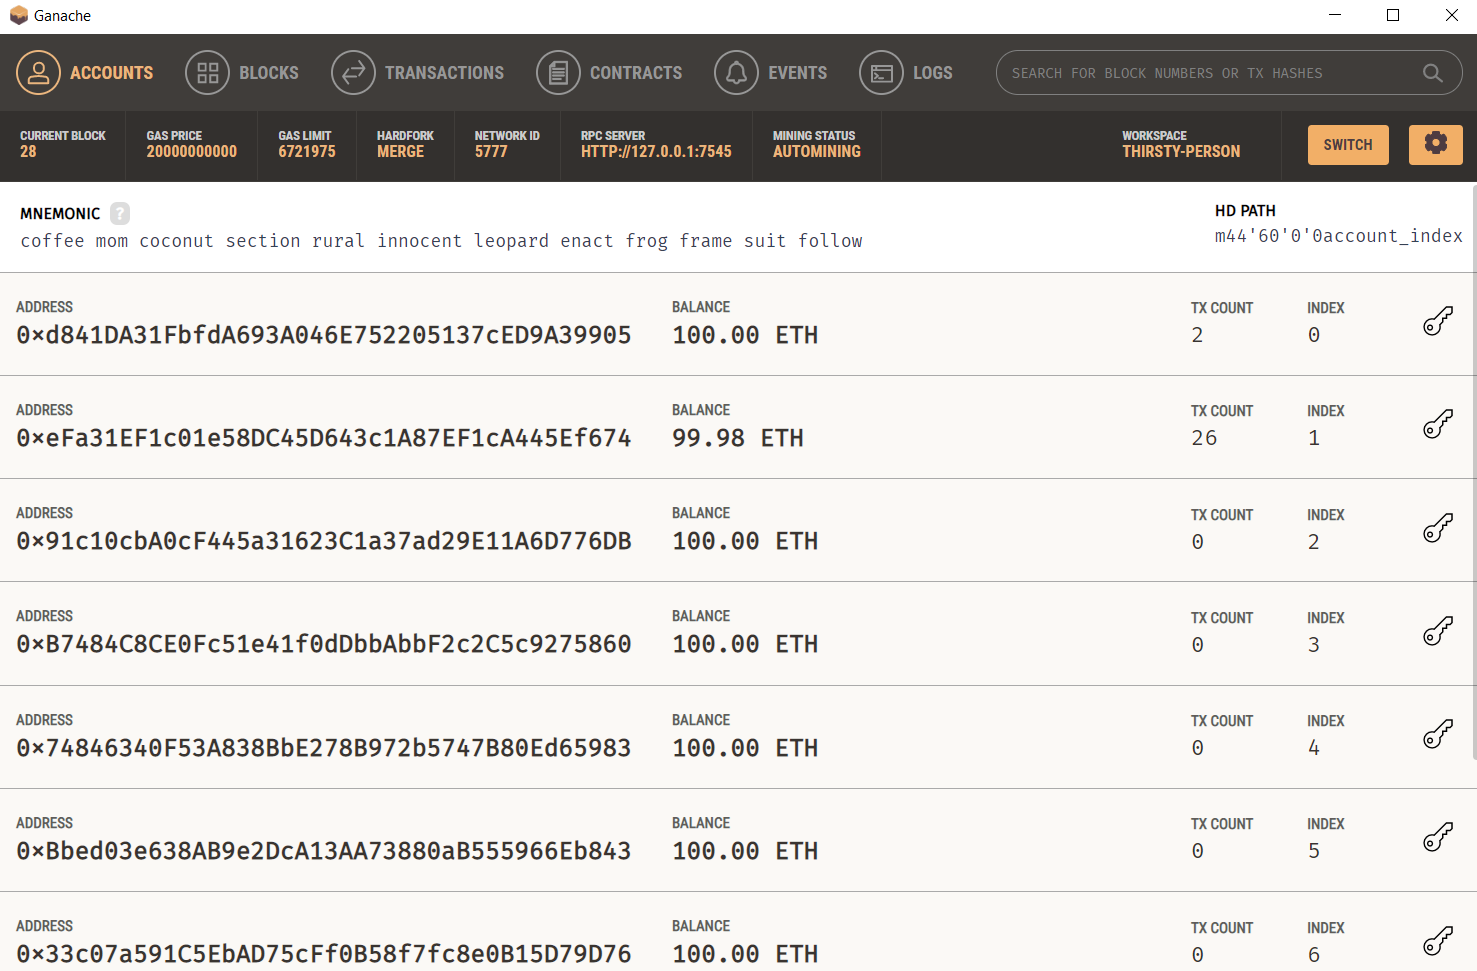
\includegraphics[width=0.8\textwidth]{chain.PNG}
\caption{Pre-funded accounts in Ganache}
\label{fig:ganache_accounts}
\end{figure}

One of the key aspects analyzed using Ganache was gas estimation. Every smart contract function consumes gas, and understanding the cost of each action is crucial for optimization. Before deploying the contract to an actual testnet, modifications were made to minimize gas expenses using Ganache's transaction cost analysis, as shown in Figure~\ref{fig:ganache_transactions}.

\begin{figure}[H]
\centering
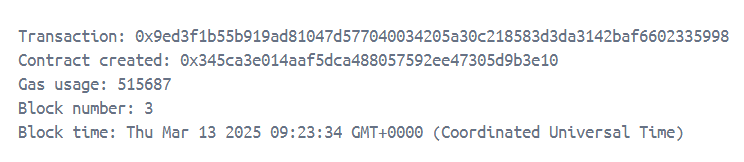
\includegraphics[width=0.8\textwidth]{contract creation.PNG}
\caption{Transaction log in Ganache showing contract creation and function execution}
\label{fig:ganache_transactions}
\end{figure}

Additionally, Ganache's instant transaction mining allowed for rapid testing iterations. Unlike Sepolia, where transactions take time to confirm, Ganache ensured that tests could be conducted quickly, leading to shorter development cycles. Figure~\ref{fig:ganache_blocks} illustrates the blockchain view in Ganache, showing the sequence of transactions and blocks mined during testing.

\begin{figure}[H]
\centering
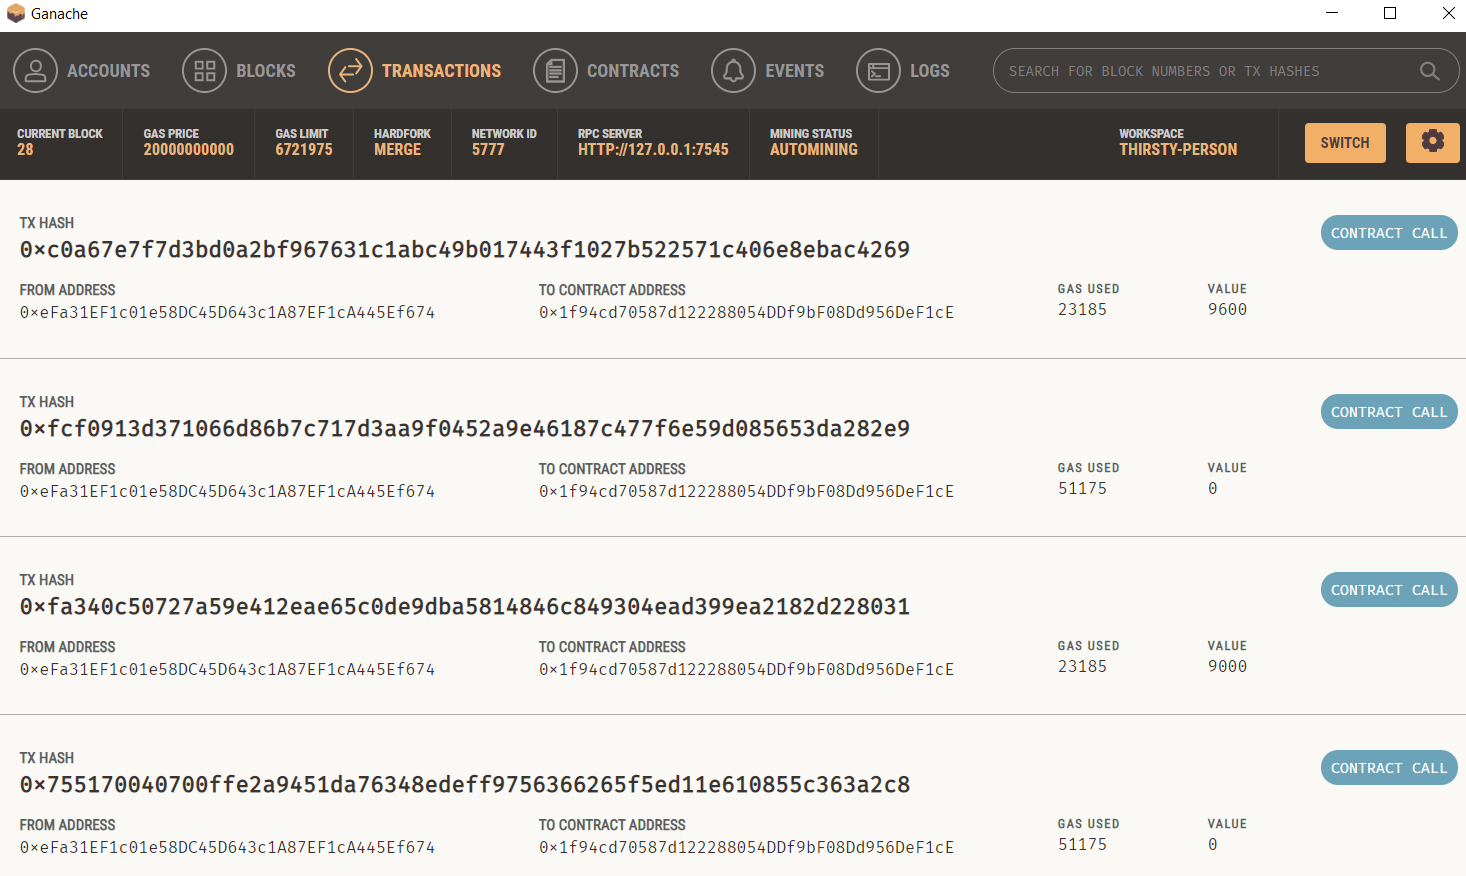
\includegraphics[width=0.8\textwidth]{trasnsactions.PNG}
\caption{Blockchain view in Ganache displaying mined blocks and transactions}
\label{fig:ganache_blocks}
\end{figure}


\section{Conclusion}
Ganache is essential for Ethereum smart contract development because it provides a rapid, reliable, and cost-free testing environment.  While testnets such as Sepolia are required for final testing prior to mainnet deployment, they present issues such as procuring test ETH and coping with network latency.  Ganache addresses these concerns by offering a local blockchain with instant transactions, pre-funded accounts, and the option to reset the blockchain state.


\chapter{Building the Web3 Application}
\section{Introduction}
The Internet has grown from a basic information-sharing platform to a global network that connects billions of people\cite{aria2023influential}\cite{nabben2023web3}\cite{murray2023promise}.  Web3 is emerging as the next phase, using blockchain technology to improve security, privacy, and user control\cite{tennakoon2023smart}\cite{sadowski2023expansive}.

 Unlike previous centralized systems, Web3 allows for direct peer-to-peer connections, decreasing dependency on middlemen.  It enables innovations such as decentralized apps (dApps), decentralized finance (DeFi), NFTs, and DAOs, which alter businesses\cite{cong2023inclusion}.

 Despite its potential, Web3 confronts obstacles such as scalability, restrictions, and environmental effect that must be addressed before widespread implementation\cite{lacity2023quiet}\cite{wang2023novel}.  This assessment examines Web3's accomplishments, prospects, and challenges, providing insight into its future.

 \section{Project Setup}
 We start by setting up a React project using Vite and installing the necessary dependencies:
 
 \begin{lstlisting}
 npm create vite@latest web3-app --template react
 cd web3-app
 npm install
 npm install web3 dotenv
 \end{lstlisting}
 
 \section{Connecting to Blockchain}
 We use Web3.js to interact with a smart contract deployed on Ganache. The connection is initialized using environment variables:
 
 \begin{lstlisting}
 import Web3 from "web3";
 
 const web3 = new Web3(import.meta.env.VITE_GANACHE_RPC);
 const contractAddress = import.meta.env.VITE_CONTRACT_ADDRESS;
 const privateKey = import.meta.env.VITE_PRIVATE_KEY;
 const account = import.meta.env.VITE_ACCOUNT;
 \end{lstlisting}
 
 \section{Fetching Energy Data}
 To get energy consumption data, we retrieve it from ThingsBoard using an API call:
 
 \begin{lstlisting}
 async function fetchEnergyData() {
     const response = await fetch(
         `http://localhost:9090/api/plugins/telemetry/DEVICE/${DEVICE_ID}/values/timeseries?keys=power`,
         { headers: { "X-Authorization": `Bearer ${thingsboardToken}` } }
     );
     const data = await response.json();
     const power = data.power[0].value;
     setEnergy(Math.floor(power));
 }
 \end{lstlisting}
 
 \section{Interacting with the Smart Contract}
 Our smart contract supports three main functions: storing energy data, fetching the bill, and making payments.
 
 \subsection{Storing Energy Data}
 The energy data is sent to the blockchain using the `storeEnergy` function:
 
 \begin{lstlisting}
 async function sendEnergyData() {
     const tx = contract.methods.storeEnergy(energy);
     const gas = await tx.estimateGas({ from: account });
     const gasPrice = await web3.eth.getGasPrice();
     const data = tx.encodeABI();
     const nonce = await web3.eth.getTransactionCount(account, "latest");
 
     const signedTx = await web3.eth.accounts.signTransaction(
         { to: contractAddress, data, gas, gasPrice, nonce },
         privateKey
     );
 
     await web3.eth.sendSignedTransaction(signedTx.rawTransaction);
 }
 \end{lstlisting}
 
 \subsection{Fetching and Paying Bills}
 To check the pending bill amount:
 
 \begin{lstlisting}
 async function fetchBill() {
     const billAmount = await contract.methods.getBill().call({ from: account });
     setBill(billAmount);
 }
 \end{lstlisting}
 
 To pay the bill using the `payBill` function:
 
 \begin{lstlisting}
 async function payBill() {
     const billAmount = await contract.methods.getBill().call({ from: account });
     const tx = contract.methods.payBill();
     const gas = await tx.estimateGas({ from: account, value: billAmount });
     const gasPrice = await web3.eth.getGasPrice();
     const data = tx.encodeABI();
     const nonce = await web3.eth.getTransactionCount(account, "latest");
 
     const signedTx = await web3.eth.accounts.signTransaction(
         { to: contractAddress, data, gas, gasPrice, nonce, value: billAmount },
         privateKey
     );
 
     await web3.eth.sendSignedTransaction(signedTx.rawTransaction);
 }
 \end{lstlisting}
 
 \section{Frontend Interface}
 The React frontend provides buttons to interact with the smart contract:
 
 \begin{lstlisting}
 return (
   <div className="container">
     <h1>Energy Billing System</h1>
     <p>Energy: {energy !== null ? `${energy} kWh` : "Fetching..."}</p>
     <p>Bill: {bill !== null ? `${bill} wei` : "Not Fetched"}</p>
     
     <button onClick={sendEnergyData}>Store Energy</button>
     <button onClick={fetchBill}>Fetch Bill</button>
     <button onClick={payBill}>Pay Bill</button>
   </div>
 );
 \end{lstlisting}
 The frontend allows seamless interaction with the smart contract, enabling users to track their energy consumption and settle their bills efficiently. The main interface of the React application is shown in Figure~\ref{fig:frontend_ui}.

\begin{figure}[H]
\centering
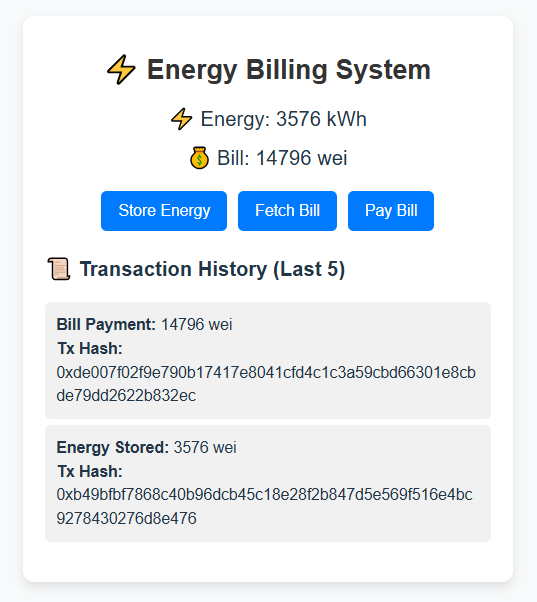
\includegraphics[width=0.4\textwidth]{web3 App.PNG}
\caption{User interface of the Energy Billing System}
\label{fig:frontend_ui}
\end{figure}

\section{Transaction Logs and User Interaction}
To verify the proper execution of smart contract functions, transaction logs from the frontend interactions were analyzed. When a user stores energy data, retrieves the bill, or makes a payment, corresponding transactions are recorded on the blockchain. Figure~\ref{fig:frontend_transactions} presents a transaction log demonstrating these interactions.

\begin{figure}[H]
\centering
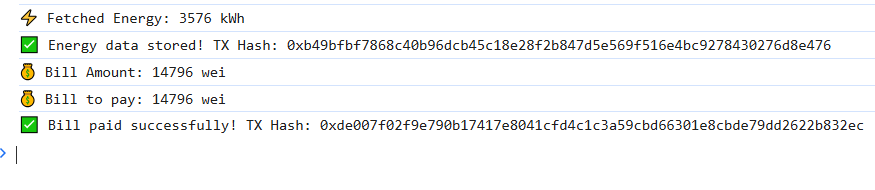
\includegraphics[width=0.8\textwidth]{frontend Logs.PNG}
\caption{Transaction log from frontend interactions with the smart contract}
\label{fig:frontend_transactions}
\end{figure}

By integrating React with Web3.js, users can seamlessly communicate with the Ethereum blockchain, ensuring a smooth and responsive experience.
 
 \section{Conclusion}
 This Web3 application successfully integrates React, Ganache, and ThingsBoard to enable decentralized energy billing. It demonstrates the potential of blockchain for transparent and automated energy management.

\chapter{Dockerizing the Complete System}
\section{Introduction}
Docker is an open-source platform that provides lightweight virtualization via Linux Containers (LXC). Docker containers, unlike typical virtual machines, share the host operating system kernel, which improves efficiency and portability. Namespaces for process separation, cgroups for resource management, and union file systems such as OverlayFS for efficient storage are all important technologies.

Docker provides consistency across environments by packaging applications alongside their dependencies\cite{dana2011}, making it perfect for microservices, CI/CD pipelines, and cloud deployments \cite{marzolla2011}.  Its scalability and low overhead have transformed modern DevOps procedures\cite{zhang2011}.

\section{Dockerization Process}

Dockerization is the process of packaging an application and its dependencies into a container. It simplifies deployment, ensures consistency across environments, and facilitates scaling. In this project, we use Docker to containerize three main components: Ganache, ThingsBoard, and a React application.

\subsection{Docker Compose}

To orchestrate multiple containers, we use Docker Compose. The following YAML configuration defines the services required for this setup:

\begin{lstlisting}[language=python]
version: '3.8'

services:
  ganache:
    image: trufflesuite/ganache
    container_name: ganache
    restart: always
    ports:
      - "8545:8545"
    command: ["--db", "/ganache-data", "--mnemonic", "candy maple cake sugar pudding cream honey rich smooth crumble sweet treat"]
    volumes:
      - ganache_data:/ganache-data
    networks:
      - app_network

  thingsboard:
    image: thingsboard/tb-postgres
    container_name: thingsboard
    restart: always
    ports:
      - "9090:9090"
      - "1883:1883" # MQTT
      - "5683:5683/udp" # CoAP
    environment:
      - DATABASE_TS_TYPE=sql
      - HTTP_CORS_ALLOW_ORIGIN=*  # Enable CORS for ThingsBoard
    volumes:
      - tb-data:/data
      - tb-logs:/var/log/thingsboard
    networks:
      - app_network

  react-app:
    build:
      context: .
      dockerfile: Dockerfile
    container_name: react-app
    restart: always
    ports:
      - "80:80"
    depends_on:
      - ganache
      - thingsboard
    env_file:
      - .env
    networks:
      - app_network

networks:
  app_network:
    driver: bridge

volumes:
  ganache_data:
  tb-data:
  tb-logs:
\end{lstlisting}

\noindent
This configuration defines the following services:
\begin{itemize}
    \item \textbf{Ganache:} A blockchain development tool for Ethereum.
    \item \textbf{ThingsBoard:} An IoT platform for data management.
    \item \textbf{React App:} A front-end web application served using Nginx.
\end{itemize}

All services are connected using a shared network, \texttt{app\_network}, ensuring seamless inter-container communication.

\subsection{Dockerfile}

The front-end React application is built using a multi-stage process. The following \texttt{Dockerfile} specifies how the React app is built and served with Nginx:

\begin{lstlisting}[language=python]
# Stage 1: Build React App with Vite
FROM node:18 AS build
WORKDIR /app
COPY package.json package-lock.json ./
RUN npm install
COPY . . 
RUN npm run build

# Stage 2: Serve with Nginx
FROM nginx:alpine
COPY --from=build /app/dist /usr/share/nginx/html
EXPOSE 80
CMD ["nginx", "-g", "daemon off;"]
\end{lstlisting}

\noindent
The build process follows two stages:
\begin{enumerate}
    \item In the first stage, Node.js is used to install dependencies and build the React application.
    \item In the second stage, the built application is copied into an Nginx container to serve it efficiently.
\end{enumerate}

\subsection{Running the Containers}

Once the configuration is complete, the following command is used to start all containers:

\begin{lstlisting}[language=bash]
docker-compose up -d
\end{lstlisting}

To verify that the containers are running, use:

\begin{lstlisting}[language=bash]
docker ps
\end{lstlisting}

If there are updates to the React application or other services, rebuild and restart the containers using:

\begin{lstlisting}[language=bash]
docker-compose up --build -d
\end{lstlisting}
\begin{figure}[H]
    \centering
    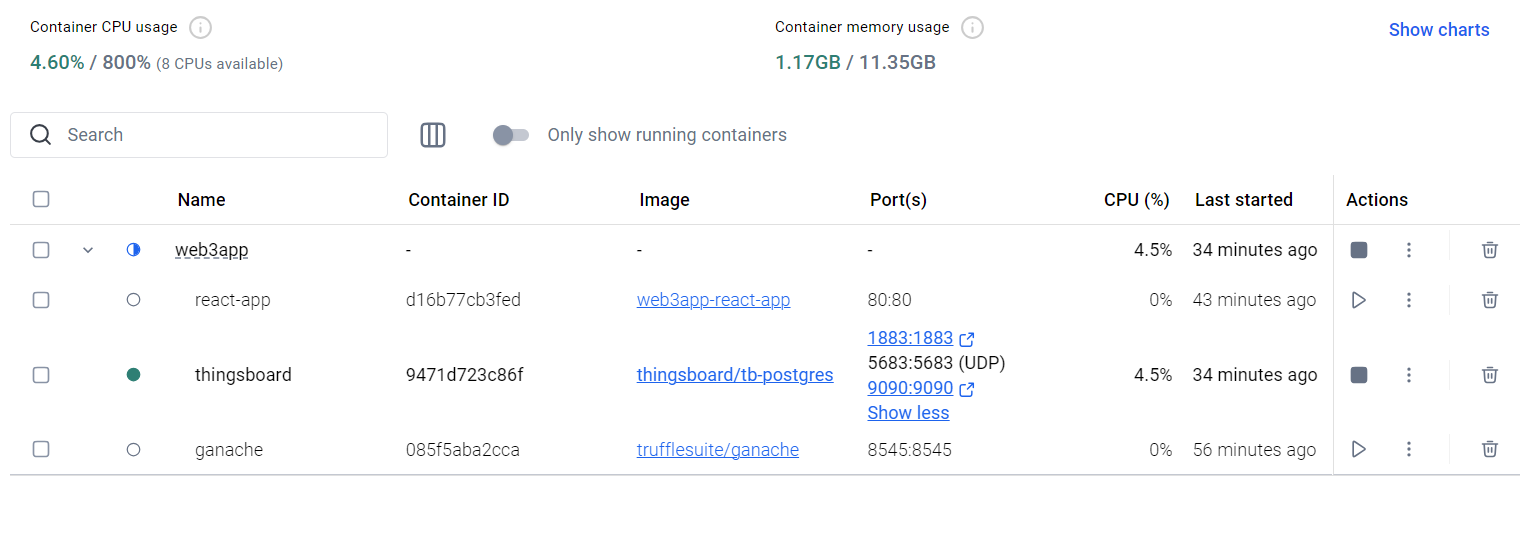
\includegraphics[width=1\textwidth]{docker container.PNG}
    \caption{Docker Containers}
    \end{figure}

\subsection{Stopping and Removing Containers}

To stop all running containers, use:

\begin{lstlisting}[language=bash]
docker-compose down
\end{lstlisting}

To remove all containers, networks, and volumes, use:

\begin{lstlisting}[language=bash]
docker-compose down -v
\end{lstlisting}

\section{Conclusion}

Dockerization provides a scalable and efficient way to manage applications by encapsulating dependencies in containers. It simplifies deployment, ensures consistency across environments, and allows for seamless integration between components. By using Docker Compose, we streamline the management of multiple services, making the development and deployment process more efficient.

\chapter{Future Scope}
The proposed smart home automation system can be improved by incorporating advanced technologies and improving its capabilities.  One important enhancement is the incorporation of smart grid technology, which enables homeowners to share excess solar energy with neighbors via blockchain-based smart contracts.  This peer-to-peer energy trading model improves energy efficiency and encourages sustainable living.  Furthermore, demand-response systems can be used to optimize energy consumption based on real-time grid circumstances, resulting in improved load management and less energy waste.
Another area for improvement is the combination of solar energy with water pumping systems.  By adding solar panel monitoring, the system can effectively measure energy generation and automate energy distribution to various home appliances.  Smart water pumping systems can also be incorporated to efficiently regulate water usage, resulting in optimal operation based on energy supply and demand.  This not only minimizes reliance on traditional power sources, but also fosters a self-sustaining smart home ecosystem.

Furthermore, upgrading to a sophisticated microcontroller with built-in Wi-Fi, such as the ESP32 or other IoT-enabled hardware, can considerably boost system performance.  These microcontrollers outperform the Raspberry Pi in terms of processing power, connectivity, and power consumption, making them perfect for real-time IoT applications.  The use of such hardware would improve the scalability, efficiency, and ease of deployment of future smart home automation solutions.


\chapter{Conclusion}
The integration of IoT, blockchain, and smart energy management into home automation has the potential to transform how energy is consumed and billed.  This project uses a decentralized approach to assure openness, security, and efficiency in energy transactions while eliminating reliance on intermediaries.  Smart contracts simplify billing processes, making energy management more efficient and cost-effective.

Looking ahead, adding community energy sharing, solar and water management, and better microcontrollers will improve the system's capabilities and practicality.  As smart homes evolve, integrating more sustainable and intelligent solutions will result in a more efficient and environmentally friendly future.  This project is a first step toward a completely automated and decentralized smart energy management system, paving the door for future advancements in home automation and energy distribution.


\newpage
% References
\renewcommand{\bibname}{References}

\bibliographystyle{IEEEtran}
\bibliography{references}

\end{document}


